\documentclass[journal,twoside]{IEEEtran}
\usepackage{cite}
\usepackage{amsmath,amssymb,amsfonts}
\usepackage{algorithm}
\usepackage{algpseudocode}
\usepackage{booktabs}
\usepackage{graphicx}
\usepackage{textcomp}
\usepackage{multirow}
\usepackage{array}
\usepackage{xcolor}
\usepackage{url}

% Visible placeholder for every number that depends on the new (MPCE) runs.
% (an empty argument, used in table cells, prints just [TBD])
\newcommand{\TBD}[1]{\textcolor{red}{[TBD\ifx\relax#1\relax\else: #1\fi]}}

\markboth{Journal of Modern Power Systems and Clean Energy, VOL. XX, NO. XX, XXXX}
{SOLANKI \MakeLowercase{\textit{et al.}}: TWO-PHASE SALP SWARM AND VARIABLE NEIGHBORHOOD SEARCH FOR WIND FARM LAYOUT OPTIMIZATION}

\begin{document}

\title{A Two-Phase Salp Swarm and Variable Neighborhood Search Algorithm for Continuous Wind Farm Layout Optimization}
\author{Prince~Solanki, Pulkit~Dwivedi, Vanita~Garg, and Vinay~Shukla
\thanks{Manuscript received: \TBD{date}; revised: \TBD{date}; accepted: \TBD{date}.}
\thanks{\TBD{funding statement, e.g., ``This work did not receive any specific grant from funding agencies.''}}
\thanks{P. Solanki \TBD{mark corresponding author} is with the Department of Mathematics, School of Sciences, IILM University, Greater Noida, Uttar Pradesh, India; he was previously with the Department of Mathematics, Indian Institute of Technology Roorkee, Roorkee, India (e-mail: prince@ma.iitr.ac.in; prince@iilm.edu).}
\thanks{P. Dwivedi is with the Department of Computer Science and Engineering, Bennett University, Greater Noida, Uttar Pradesh, India (e-mail: pdwivedi19900@gmail.com; pulkit.dwivedi@bennett.edu.in).}
\thanks{V. Garg is with Amity University, Noida, Uttar Pradesh, India (e-mail: vanitagarg16@gmail.com).}
\thanks{V. Shukla is with the School of Mathematical Sciences, Shanghai Jiao Tong University, Shanghai 200240, China, and also with the Department of Mathematics, School of Computer Science Engineering and Technology, Bennett University, Greater Noida, India (e-mail: vinayshukla4321@gmail.com; vnshukla01@sjtu.edu.cn).}}

\maketitle

\begin{abstract}
The wind farm layout optimization problem (WFLOP) asks where a prescribed number of turbines should be placed to minimize wake losses while every turbine stays inside the site and keeps a minimum distance from the others. This paper proposes SSA-VNS, a two-phase algorithm for the continuous WFLOP. The standard salp swarm algorithm (SSA) explores the layout space for the first half of the evaluation budget, and the basic variable neighborhood search (VNS) then refines the best layout found by the swarm. Both phases share a penalized objective based on the Jensen wake model and direction-dependent Weibull wind data. SSA-VNS is compared with SSA, the Laplacian SSA (LX-SSA), particle swarm optimization with constriction coefficients, differential evolution, VNS and a multistart SLSQP solver on 68 benchmark cases, with 30 seed-paired runs of 6,030 objective evaluations per method and case. SSA-VNS obtains the best average rank (\TBD{avg.\ rank}) and \TBD{summary of Holm--Wilcoxon outcome and feasibility rate}. An ablation against SSA, VNS, a random-multistart VNS and LX-SSA-VNS shows that \TBD{contribution of the VNS phase and of the swarm start}, whereas the Laplace step of LX-SSA gives no measurable gain. Further tests with feasibility-preserving initialization, budgets of up to 120,030 evaluations, a 16-turbine block of the Horns Rev~1 offshore farm and the 16- and 36-turbine scenarios of IEA Wind Task~37 Case Study~1 show \TBD{one-sentence summary}. The ranking of the methods is \TBD{stable/changed} under a cubic power curve and a Gaussian wake model.
\end{abstract}

\begin{IEEEkeywords}
Wind farm layout optimization, salp swarm algorithm, variable neighborhood search, hybrid metaheuristic, wake effect.
\end{IEEEkeywords}

\section*{Nomenclature}
\addcontentsline{toc}{section}{Nomenclature}
\begin{IEEEdescription}[\IEEEusemathlabelsep\IEEEsetlabelwidth{$\xi_1,\xi_2,\xi_3$}]
\item[$B$] Budget (number of objective calls).
\item[$C_T$] Thrust coefficient.
\item[$D$, $R$] Rotor diameter and rotor radius ($D=2R$).
\item[$d_{ij}$] Downstream distance of turbine $i$ behind turbine $j$.
\item[$\Delta_{ij}$, $\Delta_i$] Velocity deficit at turbine $i$ due to turbine $j$; combined deficit at turbine $i$.
\item[$E(P_i)$] Expected power of turbine $i$ (benchmark units).
\item[$F_p$] Penalized wake loss (minimized).
\item[$f(s)$] Power curve.
\item[$\mathbf H$] Food source (best layout of the swarm).
\item[$K$, $K_{\rm G}$] Jensen wake-spreading constant; growth rate of the Gaussian wake.
\item[$k$, $k_{\max}$] Index and number of VNS neighborhoods.
\item[$\ell_{ij}$, $\ell_{\min}$] Distance between turbines $i$ and $j$; minimum spacing.
\item[$N$, $N_p$] Number of turbines; population size.
\item[$N_\theta$, $N_s$] Numbers of wind-direction and wind-speed bins.
\item[$p_l$] Probability of the $l$th wind-direction bin.
\item[$r$] Farm radius.
\item[$s$] Wind speed.
\item[$t$, $T$, $T_1$] Iteration counter, number of swarm iterations, and number of SSA iterations in Phase~1.
\item[$\mathbf X$] Layout vector $(x_1,y_1,\ldots,x_N,y_N)\in\mathbb R^{2N}$.
\item[$x_i$, $y_i$] Coordinates of turbine $i$.
\item[$\alpha$, $\beta_{ij}$] Half-cone angle of the wake; wake angle of turbine $i$ with respect to turbine $j$.
\item[$\delta_k$] Outer radius of the $k$th VNS neighborhood.
\item[$\zeta$, $\psi$] Weibull shape and scale parameters.
\item[$\theta$] Wind direction (direction the wind blows towards, counter-clockwise from east).
\item[$\lambda_1$, $\lambda_0$] Slope and intercept of the linear power curve.
\item[$\mu$] Penalty factor.
\item[$\phi$, $\chi$] Location and scale of the Laplace step (LX-SSA).
\item[$\xi_1,\xi_2,\xi_3$] SSA leader coefficient and uniform random numbers.
\item[$\omega$] Fraction of the budget given to Phase~1.
\end{IEEEdescription}

\section{Introduction}

Wind energy has become one of the main sources of low-carbon electricity. Since most of the cost of a wind project is fixed at the planning stage, the decisions taken before construction have a lasting effect on the energy a farm will deliver, and one of the most important of these decisions is where the turbines are placed.

The wind farm layout optimization problem (WFLOP) deals with exactly this question. An upstream turbine extracts momentum from the flow and leaves behind a wake of slower and more turbulent air, so that the turbines downstream produce less power. The wake widens and recovers with distance, which suggests spreading the turbines as far apart as possible. The site, however, is limited, and the turbines must keep a minimum distance from each other. The objective is nonlinear, the wakes couple the positions of all turbines, and the feasible region is bounded by many nonconvex spacing constraints. For these reasons, WFLOP has become a popular test bed for metaheuristic search.

Mosetti et al.~\cite{Mosetti1994} and Grady et al.~\cite{Grady2005} were among the first to address WFLOP, using a binary-coded genetic algorithm (GA) on a grid. Ozturk and Norman~\cite{Ozturk2004} placed turbines in continuous space with a heuristic that accounts for wind speed, wind direction and wake interactions. Lackner and Elkinton~\cite{Lackner2007} proposed an analytical model for offshore farms, Castro Mora et al.~\cite{Mora2007} designed layouts with a GA under spacing and wind-speed constraints, and Huang~\cite{Huang2007} used a distributed GA to maximize the annual profit of large farms. Elkinton et al.~\cite{Elkinton2008} compared GA, particle swarm optimization (PSO), differential evolution (DE) and simulated annealing (SA) for offshore layouts, and SA was also used by Bilbao and Alba~\cite{Bilbao2009} and by Rivas et al.~\cite{Rivas2009}.

Emami and Noghreh~\cite{Emami2010} added the construction cost to the objective, and \c{S}i\c{s}bot et al.~\cite{Sisbot2010} used a multi-objective GA to trade energy production against installation cost. Kusiak and Song~\cite{Kusiak2010} introduced the wind-distribution-based placement model that we also use. Ero\u{g}lu and Se\c{c}kiner~\cite{Eroglu2012,Eroglu2013} applied ant colony optimization (ACO) and particle filtering to the same model, Samorani~\cite{Samorani2013} studied the trade-off between power output and wake effect, and Bansal and Farswan~\cite{Bansal2017} used biogeography-based optimization and proposed an upper limit on the number of turbines for a given farm. ACO has also been used to design the collector system of offshore farms~\cite{Srikakulapu2018}.

Later studies refined both the algorithms and the models. Ju and Liu~\cite{Ju2019} proposed a self-informed GA, Jin et al.~\cite{Jin2019} optimized the cable routing of offshore plants with an adaptive PSO, and Hou et al.~\cite{Hou2019} reviewed layout and electrical-system design. Dhiman et al.~\cite{Dhiman2020} used lidar data to steer the wakes, Nagpal et al.~\cite{Nagpal2021} refined GA layouts with continuous local methods, and PSO has been applied to reduce wake losses~\cite{Asaah2021}. Bai et al.~\cite{Bai2022} integrated Monte Carlo tree search into an adaptive GA, and Cazzaro and Pisinger~\cite{Cazzaro2022} developed a variable neighborhood search (VNS) heuristic for large offshore farms. Pseudo-gradient methods~\cite{Quaeghebeur2021}, three-dimensional Gaussian wake models~\cite{Tao2020}, and machine-learning~\cite{Yang2023}, CFD-based Kriging~\cite{Wang2024} and data-driven or physics-informed~\cite{Yang2024,Li2025} surrogates have also been introduced. The IEA Wind Task~37 layout optimization case study~\cite{Baker2019} showed that, even with a common wake model, different optimizers reach clearly different layouts. No single optimizer or wake model dominates this literature.

Swarm methods such as the salp swarm algorithm (SSA)~\cite{Mirjalili2017} are attractive for WFLOP because they are simple and cheap per iteration. In earlier work, two of the authors introduced the Laplacian SSA (LX-SSA)~\cite{Solanki2023}, in which each follower salp also tries a Laplace-distributed move relative to the food source. In WFLOP, however, we observed that a swarm spends most of the second half of its budget on small improvements once it has contracted around the best layout, because the final refinement of a layout requires coordinated moves of single turbines along the spacing constraints. Trajectory methods such as VNS~\cite{Mladenovic1997,Hansen2001} behave the other way round: they refine one layout efficiently by alternating random perturbations of growing size with a local search, but the result depends on where the search starts.

This complementary behavior motivates the present work. We propose SSA-VNS, a two-phase algorithm in which the standard SSA explores the layout space for the first half of the evaluation budget and the basic VNS then refines the best layout found by the swarm. We first built the hybrid on LX-SSA. In our runs, however, the Laplace step did not help: LX-SSA-VNS was never significantly better than SSA-VNS (Section~\ref{sec:ablation}). The proposed method therefore uses the standard SSA; LX-SSA is kept as a baseline and LX-SSA-VNS as an ablation variant. We keep the standard ingredients of the benchmark, namely the Jensen wake model, a Weibull description of the wind and the Kusiak--Song power model, so that the results can be compared with the earlier literature, and we examine the effect of these choices separately. Our contributions are as follows:
\begin{enumerate}
\item We propose SSA-VNS, a two-phase algorithm for the continuous WFLOP with explicit boundary and minimum-spacing constraints, in which both phases share one penalized objective (Section~\ref{sec:hybrid}).
\item We compare SSA-VNS with SSA, LX-SSA, PSO with constriction coefficients, DE, VNS and a gradient-based multistart SLSQP solver on 68 benchmark cases at equal numbers of objective evaluations, with 30 seed-paired runs per method and case, Friedman and Holm-corrected Wilcoxon tests, feasibility rates and convergence curves (Section~\ref{sec:results}).
\item We carry out an ablation that isolates the VNS phase, the value of the swarm start (against VNS from the best initial point and against a random-multistart control, RS-VNS), the Laplace step (LX-SSA-VNS) and the budget split (Section~\ref{sec:ablation}).
\item We test the methods beyond the benchmark: with feasibility-preserving initialization, with budgets of up to 120,030 evaluations, on a 16-turbine block of the Horns Rev~1 offshore farm, on the 16- and 36-turbine scenarios of IEA Wind Task~37 Case Study~1 (IEA37) against the published results, and under alternative power-curve, wake, spacing and boundary assumptions (Sections~\ref{sec:beyond} and~\ref{sec:robustness}).
\end{enumerate}

Section~\ref{sec:model} describes the WFLOP model and the constraint handling, Section~\ref{sec:ssa} summarizes SSA and LX-SSA, and Section~\ref{sec:hybrid} introduces SSA-VNS. Section~\ref{sec:setup} describes the experimental setup. Sections~\ref{sec:results} and~\ref{sec:beyond} report the results on the benchmark and beyond it, Section~\ref{sec:robustness} examines the sensitivity to the modeling assumptions, and Section~\ref{sec:limits} states the limitations. Section~\ref{sec:conclusion} concludes the paper.

\section{Problem Modeling}
\label{sec:model}

We use the following definitions and assumptions.
\begin{enumerate}
    \item \textbf{Prescribed turbine count:} In every run the number of turbines $N$ is fixed in advance, and only the $2N$ turbine coordinates are optimized. Results for several values of $N$ form a sweep over the turbine count; $N$ and the positions are not optimized jointly.
    \item \textbf{Turbine location:} Turbine $i$ is located by its planar coordinates $(x_i,y_i)$, measured from the center of the farm.
    \item \textbf{Identical turbines:} All turbines have the same power curve, rated power, rotor size and hub height.
    \item \textbf{Wind speed:} For a given wind direction, the wind speed $s$ follows a Weibull distribution with density
    \[
        p_s (s;\zeta,\psi) = \frac{\zeta}{\psi} \left( \frac{s}{\psi} \right)^{\zeta-1} \exp\left[-\left( \frac{s}{\psi} \right)^\zeta \right],
    \]
    where $\zeta$ is the shape and $\psi$ the scale parameter.
    \item \textbf{Wind direction:} Both Weibull parameters depend on the wind direction $\theta$, i.e., $\zeta=\zeta(\theta)$ and $\psi=\psi(\theta)$, $0^\circ\le\theta<360^\circ$. Throughout the paper, $\theta$ is the direction \emph{towards} which the wind blows, measured counter-clockwise from east (Fig.~\ref{fig:wind farm}): $\theta=0^\circ$ points east and $90^\circ$ north, and turbine $i$ lies downstream of turbine $j$ when $(x_i-x_j)\cos\theta+(y_i-y_j)\sin\theta>0$. The benchmark wind data (Table~\ref{tab:wind}) are used in this convention, as in the benchmark implementation. Meteorological directions $\varphi$ (the direction the wind comes \emph{from}, clockwise from north), as given for Horns Rev~1 and IEA37, are converted by $\theta=270^\circ-\varphi$.
    \item \textbf{Minimum spacing:} Any two turbines must be at least $\ell_{\min}=4D=8R$ apart, where $D=2R$ is the rotor diameter:
    $\ell_{ij}=\sqrt{(x_i - x_j)^2 + (y_i - y_j)^2} \geq \ell_{\min}$.
    This is the value adopted in the benchmark studies~\cite{Kusiak2010,Bansal2017}. Real projects often require larger distances; Section~\ref{sec:spacing} studies $5D$ and $6D$.
    \item \textbf{Farm boundary:} The farm is circular, as in~\cite{Kusiak2010,Bansal2017}, and every turbine must satisfy $x_i^2 + y_i^2 \leq r^2$. We study farms with $r=500$, 750 and 1000~m. The search space is continuous, so the turbines are not restricted to the nodes of a grid.
    \item \textbf{Model and objective:} We use the Jensen wake model~\cite{Jensen1983, Katic1986} and the power model of Kusiak and Song~\cite{Kusiak2010}. The aim is to maximize the expected power of the farm, i.e., to minimize the wake losses, subject to the spacing and boundary constraints.
\end{enumerate}

\begin{figure}[!t]
\centering
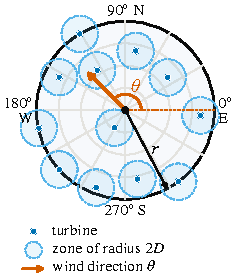
\includegraphics[width=0.9\columnwidth]{figures_final/fig_wind_farm.pdf}
\caption{Circular wind farm of radius $r$. The wind direction $\theta$ (direction the wind blows towards) is measured counter-clockwise from east. The points show the best \TBD{regenerate with the best SSA-VNS layout} layout for 12 turbines in the 750-m farm (Wind Data Set~I); the shaded discs have radius $2D$, so two discs touch when their turbines are exactly $4D$ apart.}
\label{fig:wind farm}
\end{figure}

\subsection{Wake Effect Model}

In the Jensen model~\cite{Jensen1983,Katic1986}, the wake behind a rotor expands linearly with the downstream distance, and the wind speed inside it drops from the upstream value $s_{\text{up}}$ to $s_{\text{down}}$ (Fig.~\ref{fig:wake-model}). Let $K$ be the wake-spreading constant and $d_{ij}$ the distance of turbine $i$ behind turbine $j$ along the wind direction. The velocity deficit at turbine $i$ due to the wake of turbine $j$ is
\begin{equation}
    \Delta_{ij} = 1-\frac{s_{\text{down}}}{s_{\text{up}}}=\frac{1 - \sqrt{1 - C_T}}{\left(1 + K d_{ij}/R\right)^2},
    \label{eq:deficit}
\end{equation}
where $C_T$ is the thrust coefficient. Gaussian and three-dimensional wake models describe the velocity field more realistically~\cite{Tao2020,Cao2022}; Section~\ref{sec:powercurve} therefore re-evaluates all optimized layouts with a Gaussian model.

\begin{figure}[!t]
\centering
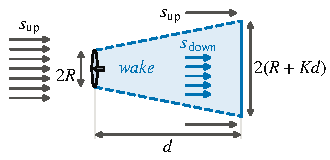
\includegraphics[width=0.9\columnwidth]{figures_final/fig_wake_model.pdf}
\caption{Jensen wake behind a rotor of radius $R$ (schematic, not to scale). The wake widens linearly with the spreading constant $K$, so that its width at the downstream distance $d$ is $2(R+Kd)$, and the wind speed inside it drops from $s_{\text{up}}$ to $s_{\text{down}}$.}
\label{fig:wake-model}
\end{figure}

The wake of turbine $j$ is idealized as a half cone whose virtual vertex $A$ lies a distance $R/K$ upstream of the rotor (Fig.~\ref{fig:half-cone}); its half-cone angle is $\alpha=\arctan K$. Whether turbine $i$ lies in this cone is decided by the following two definitions.

\begin{figure}[!t]
\centering
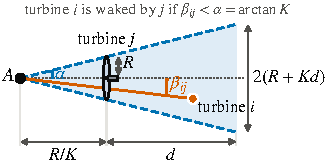
\includegraphics[width=0.9\columnwidth]{figures_final/fig_half_cone.pdf}
\caption{Wake half cone of turbine $j$ (schematic, $K$ exaggerated). The virtual vertex $A$ lies a distance $R/K$ upstream of the rotor, the half-cone angle is $\alpha=\arctan K$, and a downstream turbine $i$ lies in the wake of $j$ when $\beta_{ij}<\alpha$.}
\label{fig:half-cone}
\end{figure}

\textbf{Definition 1 (wake angle).} For a wind direction $\theta$, the wake angle $\beta_{ij}\in[0,\pi]$ is the angle at the vertex $A$ of the wake of turbine $j$ between the wake axis and the line from $A$ to turbine $i$:
\[
\beta_{ij} = \cos^{-1}\!\left(\frac{u_{ij}}{\sqrt{u_{ij}^2+v_{ij}^2}}\right),
\]
with
\begin{align*}
u_{ij}&=(x_i - x_j)\cos\theta + (y_i - y_j)\sin\theta + R/K,\\
v_{ij}&=-(x_i - x_j)\sin\theta + (y_i - y_j)\cos\theta ,
\end{align*}
where $v_{ij}$ is the lateral offset of turbine $i$ from the wake axis of turbine $j$.

\textbf{Definition 2 (downstream distance).} The distance of turbine $i$ behind turbine $j$ along the wind direction $\theta$ is
$d_{ij} = \left| (x_i - x_j)\cos\theta + (y_i - y_j)\sin\theta \right|$.

Turbine $i$ lies in the wake of turbine $j$ if $\beta_{ij}<\alpha$. The deficits at turbine $i$ are combined by the root-sum-square rule over all turbines whose wake contains it:
\begin{equation}\label{eq5}
\Delta_i(\theta) = \sqrt{ \sum_{j \ne i,\ \beta_{ij} < \alpha} \Delta_{ij}^2 } .
\end{equation}

The deficit enters the energy calculation through the Weibull scale parameter. In the benchmark, $\Delta_i(\theta)$ acts as a fixed multiplicative reduction of the free-stream speed within a direction bin. Since $aS\sim\mathrm{Weibull}(\zeta,a\psi)$ for any constant $a>0$ when $S\sim\mathrm{Weibull}(\zeta,\psi)$, the local wind speed at turbine $i$ keeps the shape parameter and has the scale parameter
\begin{align}
\psi_i(\theta) &= \psi(\theta)\left[1-\Delta_i(\theta)\right],
\quad i=1,2,\ldots,N. \label{eq:weibull-scale}
\end{align}

\subsection{Power Model}
\label{sec:powermodel}

We use the power curve of the Kusiak--Song benchmark~\cite{Kusiak2010},
\begin{align}\label{eq7}
f(s) =
\begin{cases}
0, & s < s_{\text{cut-in}},\\
\lambda_1 s + \lambda_0, & s_{\text{cut-in}} \leq s \leq s_{\text{rated}},\\
P_{\text{rated}}, & s > s_{\text{rated}},
\end{cases}
\end{align}
with $s_{\text{cut-in}}=3.5$~m/s, $s_{\text{rated}}=14$~m/s, $P_{\text{rated}}=1500$~kW, $\lambda_1=140.86$ and $\lambda_0=-500$. We use this curve exactly as published, although it is not continuous: its linear part is slightly negative just above the cut-in speed ($-7.0$~kW at 3.5~m/s, zero at 3.55~m/s) and reaches 1472~kW at the rated speed, where it jumps to 1500~kW. The benchmark has no cut-out speed. Section~\ref{sec:powercurve} re-evaluates all layouts with a cubic power curve, with and without a 25~m/s cut-out.

The expected power of turbine $i$ is
\begin{equation}\label{eq8}
E(P_i) = \int_0^{360} p_\theta(\theta) \int_0^{\infty} f(s)\,
       p_s\bigl(s; \zeta(\theta), \psi_i(\theta)\bigr) \, ds \, d\theta ,
\end{equation}
where $p_\theta$ is the probability density of the wind direction. Following~\cite{Kusiak2010}, the integrals are evaluated with a Riemann sum~\cite{Stroock1999}. The wind direction is divided into bins $\theta_0 = 0^\circ, \theta_1, \ldots, \theta_{N_\theta} = 360^\circ$ with probabilities $p_l$ and the speed range between $s_{\text{cut-in}}$ and $s_{\text{rated}}$ into bins $s_0 = s_{\text{cut-in}}, s_1, \ldots, s_{N_s} = s_{\text{rated}}$. With $\bar\theta_l=(\theta_{l-1}+\theta_l)/2$ and $W_i(s,\theta)=\exp\{-[s/\psi_i(\theta)]^{\zeta(\theta)}\}$,
{\small
\begin{align*}
E(P_i) ={}& \sum_{l=1}^{N_\theta} (\theta_l - \theta_{l-1})\, p_l \Bigg\{ P_{\text{rated}}\, W_i(s_{\text{rated}},\bar\theta_l)\\
&+\lambda_1 \sum_{q=1}^{N_s} \frac{s_{q-1} + s_q}{2}\left[W_i(s_{q-1},\bar\theta_l)-W_i(s_q,\bar\theta_l)\right]\\
&+ \lambda_0 \left[W_i(s_{\text{cut-in}},\bar\theta_l)-W_i(s_{\text{rated}},\bar\theta_l)\right] \Bigg\}.
\end{align*}
}

\paragraph*{Benchmark objective and energy}
Like the earlier studies, we keep the bin-width factor $(\theta_l-\theta_{l-1})$ in the sum. Because all 24 direction bins are $15^\circ$ wide and $\sum_l p_l=1$, the objective equals 15 times the expected farm power in kW, and the annual energy production follows as $\mathrm{AEP}\,[\mathrm{MWh}] = (\text{objective}/15)\times 8.76$. For example, the wake-free objective of a single turbine under Wind Data Set~I is $14045.74$, which corresponds to an expected power of $936.38$~kW, a capacity factor of $0.624$ and an AEP of $8202.7$~MWh.

\subsection{Constraint Handling}
\label{sec:constraints}

Both constraints are handled by two simple operations that all penalty-based methods share. After every position update, each coordinate is clipped to the square that encloses the farm, $x_i\leftarrow\min\{\max\{x_i,-r\},r\}$ and likewise for $y_i$ (box repair). This keeps the variables bounded but does not enforce the circular boundary, which, like the spacing, is handled by a penalty. With the violations
\begin{equation}
g^{\rm s}_{ij}=\ell_{\min}-\ell_{ij},\qquad g^{\rm b}_{i}=x_i^2+y_i^2-r^2,
\label{eq:spacingviolation}
\end{equation}
a layout is feasible if $g^{\rm s}_{ij}\le0$ and $g^{\rm b}_i\le0$ for all $i$ and $j$. All penalty-based optimizers minimize the penalized wake loss
\begin{equation}
\begin{split}
F_p(\mathbf X)={}&\Bigl(N E_{\rm ideal}-\sum_{i=1}^{N}E(P_i)\Bigr)+\sum_{i:\,g^{\rm b}_i>0}\bigl(1+\mu g^{\rm b}_i\bigr)^2\\
&+\sum_{i<j:\,g^{\rm s}_{ij}>0}\bigl(1+\mu g^{\rm s}_{ij}\bigr)^2,\qquad \mu=10^{10},
\end{split}
\label{eq:penalty}
\end{equation}
where $\mathbf X=(x_1,y_1,\ldots,x_N,y_N)$ and $N E_{\rm ideal}$ is the wake-free objective, so that the first term is the wake loss reported in our tables. Any violation larger than about $10^{-7}$ (m or m$^2$) makes the penalty larger than the largest possible wake loss. Comparing $F_p$ values therefore gives a feasibility-first selection: a feasible layout is always preferred to an infeasible one, two feasible layouts are compared by their wake loss, and two infeasible layouts by their total penalty. Section~\ref{sec:boundary} shows that the boundary rule matters, so we keep it the same for all methods.

\section{Salp Swarm Algorithm and Its Laplacian Variant}
\label{sec:ssa}

The SSA~\cite{Mirjalili2017} keeps a population of $N_p$ salps, i.e., candidate vectors $\mathbf X^i\in\mathbb R^{n}$ with components $X^i_m$, $m=1,\ldots,n$, and the best solution found so far as the food source $\mathbf H$. In the implementation used here, the population is sorted by the objective and split into a leader half and a follower half. A leader salp $i\le N_p/2$ updates each coordinate around the food source,
\begin{align}\label{eq:leader}
X_m^i =
\begin{cases}
H_m+\xi_1\big((ub_m-lb_m)\xi_2+lb_m\big), & \xi_3\ge0.5,\\
H_m-\xi_1\big((ub_m-lb_m)\xi_2+lb_m\big), & \xi_3<0.5,
\end{cases}
\end{align}
where $lb_m$ and $ub_m$ are the bounds, $\xi_2,\xi_3\sim U(0,1)$ and $\xi_1=2\exp[-(4t/T)^2]$ decreases with the iteration $t$ out of $T$. A follower salp $i>N_p/2$ moves to the midpoint between itself and the preceding salp,
\begin{align}\label{eq:follower}
X_m^i\leftarrow\tfrac{1}{2}\left(X_m^i+X_m^{i-1}\right).
\end{align}
After all updates, the population is box-repaired and evaluated, which costs $N_p$ objective calls per iteration, and $\mathbf H$ is updated.

LX-SSA~\cite{Solanki2023} keeps these dynamics and gives each follower a second, Laplace-based candidate~\cite{Solanki2023,Deep2007},
\begin{align}
Y_m^i&=X_m^i+\gamma\left(H_m-X_m^i\right),\nonumber\\
\gamma&=
\begin{cases}
\phi+\chi\ln(2z), & z\le0.5,\\
\phi-\chi\ln\bigl(2(1-z)\bigr), & z>0.5,
\end{cases}\label{eq:laplace}
\end{align}
with $z\sim U(0,1)$, i.e., $\gamma$ is a Laplace variable with location $\phi$ and scale $\chi$. We use $\phi=0$ and $\chi=1$, so that $P(|\gamma|>1)=e^{-1}\approx0.37$. Because the Laplace distribution has heavier tails than a Gaussian, most candidates move towards $\mathbf H$ or away from it by a fraction of their current distance, while some move beyond $\mathbf H$ or far away from it. The follower keeps the better of its two candidates. Since each follower evaluates both candidates before the population is re-evaluated, one LX-SSA iteration costs $2N_p$ calls. Algorithm~\ref{alg:ssa} summarizes both methods; the comparison between them isolates the Laplace step.

\begin{algorithm}[!t]
\caption{SSA and LX-SSA (lines marked LX: LX-SSA only)}
\label{alg:ssa}
\begin{algorithmic}[1]
\State Draw and evaluate $N_p$ salps; sort them and set the best as food source $\mathbf H$.
\For{$t=1$ to $T$}
    \State Update $\xi_1=2\exp[-(4t/T)^2]$.
    \For{salp $i=1,\ldots,N_p$}
        \If{$i\le N_p/2$}
            \State Update leader $i$ using \eqref{eq:leader}.
        \Else
            \State Form the follower candidate using \eqref{eq:follower}.
            \State LX: form $\mathbf Y^i$ using \eqref{eq:laplace}, evaluate both candidates and keep the better one.
        \EndIf
    \EndFor
    \State Apply box repair, evaluate $F_p$ for the population, sort it, and update $\mathbf H$.
\EndFor
\State \Return $\mathbf H$.
\end{algorithmic}
\end{algorithm}

\section{Proposed SSA-VNS Algorithm}
\label{sec:hybrid}

Swarm methods spread their search over many regions of the layout space, but once the swarm has contracted around the food source, most of the remaining evaluations bring only small gains. VNS~\cite{Mladenovic1997,Hansen2001} refines a single layout systematically, but its result depends on the starting point. SSA-VNS combines the two: SSA explores the layout space, and the basic VNS refines the best layout it finds.

\subsection{Encoding and Objective}
For a prescribed turbine count $N$, a candidate is the layout vector $\mathbf X=(x_1,y_1,\ldots,x_N,y_N)\in\mathbb R^{n}$, $n=2N$, with bounds $[-r,r]^{n}$. Every candidate is box-repaired, its deficits $\Delta_i(\theta)$ and scale parameters $\psi_i(\theta)$ are computed for every direction bin by \eqref{eq5} and \eqref{eq:weibull-scale}, and $F_p$ is evaluated by \eqref{eq:penalty}. Both phases use $F_p$ in every comparison, sort and acceptance step, so the feasibility-first rules of Section~\ref{sec:constraints} hold throughout.

\subsection{Phase 1: Exploration by SSA}
For a budget of $B$ objective calls and a split fraction $\omega\in(0,1)$, SSA (Algorithm~\ref{alg:ssa}) runs with population $N_p$ for
\[
T_1=\operatorname{round}\!\left(\frac{\omega B-N_p}{N_p}\right)
\]
iterations, since the initial population costs $N_p$ calls and one SSA iteration costs another $N_p$. Its coefficient $\xi_1$ decreases over these $T_1$ iterations, so the swarm moves from exploration to exploitation within Phase~1. The food source $\mathbf H$ at the end of Phase~1 is the starting point of Phase~2.

\subsection{Phase 2: Refinement by Basic VNS}
Phase~2 is the basic VNS of Mladenovi\'c and Hansen~\cite{Mladenovic1997,Hansen2001} in the continuous form of Mladenovi\'c et al.~\cite{Mladenovic2008}, applied to $F_p$. It uses $k_{\max}=5$ nested $\ell_\infty$ neighborhoods of the whole layout,
\[
\mathcal N_k(\mathbf X)=\{\mathbf X':\delta_{k-1}<\lVert \mathbf X'-\mathbf X\rVert_\infty\le\delta_k\},\qquad \delta_k=0.1\,k\,r .
\]
In the shaking step, a point is drawn uniformly from $\mathcal N_k(\mathbf X)$, so that all $2N$ coordinates move, and box repair is applied. The shaken layout is then improved by a complete best-improvement local search. Since the top-hat Jensen wake makes $F_p$ discontinuous, we use a derivative-free compass search: it evaluates all $2n=4N$ moves $\pm h\,\mathbf e_m$ along the coordinate axes, moves to the best improving one, and halves the step $h$ (starting from $0.05r$) when no move improves, until $h<10^{-3}r$. If the resulting local minimum is better than the incumbent, it is accepted and $k$ is reset to 1; otherwise $k$ is increased by one, and it returns to 1 after $k_{\max}$. Phase~2 first applies the local search to $\mathbf H$ and then repeats shaking, local search and neighborhood change until the budget $B$ is used up. It returns the best layout evaluated. Algorithm~\ref{alg:hybrid} gives the complete procedure.

\begin{algorithm}[!t]
\caption{SSA-VNS for a prescribed turbine count $N$}
\label{alg:hybrid}
\begin{algorithmic}[1]
\Require budget $B$, split $\omega$, population $N_p$, farm radius $r$, $k_{\max}$
\State $T_1\gets\operatorname{round}((\omega B-N_p)/N_p)$
\State Run SSA (Algorithm~\ref{alg:ssa}) with $T=T_1$; let $\mathbf H$ be its food source
\State $\mathbf X\gets\textsc{LocalSearch}(\mathbf H)$; $k\gets1$
\While{fewer than $B$ objective calls have been used}
    \State $\mathbf X'\gets$ uniform random point of $\mathcal N_k(\mathbf X)$; box repair
    \State $\mathbf X'\gets\textsc{LocalSearch}(\mathbf X')$
    \If{$F_p(\mathbf X')<F_p(\mathbf X)$}
        \State $\mathbf X\gets \mathbf X'$; $k\gets1$
    \Else
        \State $k\gets k\bmod k_{\max}+1$
    \EndIf
\EndWhile
\State \Return best layout evaluated
\Statex
\Function{LocalSearch}{$\mathbf X'$} \Comment{compass search}
    \State $h\gets0.05r$
    \While{$h\ge10^{-3}r$}
        \State $\mathbf X^\star\gets\arg\min F_p$ over the $2n$ points $\mathbf X'\pm h\,\mathbf e_m$ (box-repaired)
        \If{$F_p(\mathbf X^\star)<F_p(\mathbf X')$} \State $\mathbf X'\gets \mathbf X^\star$ \Else \State $h\gets h/2$ \EndIf
    \EndWhile
    \State \Return $\mathbf X'$
\EndFunction
\end{algorithmic}
\end{algorithm}

\subsection{Parameters and Cost}
SSA-VNS uses $N_p=30$ and the VNS settings above, and it adds a single parameter, the split $\omega$. With the default $\omega=0.5$ and $B=6{,}030$, SSA runs for $T_1=100$ iterations and receives $30+100\times30=3{,}030$ calls, and VNS the remaining 3,000; the effect of $\omega$ is studied in Section~\ref{sec:ablation}. None of these values was tuned. The cost of both phases is dominated by the objective evaluations, so for a budget of $B$ calls SSA-VNS has the same $\mathcal O(B\,N^2N_\theta N_s)$ cost as the other methods; box repair, shaking and each compass move are $\mathcal O(N)$ and the spacing check $\mathcal O(N^2)$. Because the random-number generator is seeded once and Phase~1 draws the initial population first, SSA-VNS starts from the same initial population as all other methods for a given seed, which keeps the comparisons paired.

\section{Experimental Setup}
\label{sec:setup}

\subsection{Benchmark Cases}
We use the two wind data sets of Table~\ref{tab:wind}. In Wind Data Set~I, the Weibull parameters are the same in all directions ($\zeta=2$, $\psi=13$) and the wind is strongly directional ($p_6=0.2$, $p_7=0.6$). Wind Data Set~II keeps $\zeta=2$, but $\psi$ varies from 2.6 to 10 with the direction and the wind is spread over more directions. The wind direction is divided into $N_\theta=24$ bins of $15^\circ$, and the speed range from $s_{\text{cut-in}}$ to $s_{\text{rated}}$ into $N_s=21$ intervals of 0.5~m/s. Each data set is combined with three circular farms of radius $r=500$, 750 and 1000~m, with $N=2,\ldots,10$, $2,\ldots,12$ and $2,\ldots,15$ turbines, respectively, which gives $2\times(9+11+14)=68$ cases. The turbines have $R=38.5$~m, $\ell_{\min}=4D=308$~m, $C_T=0.8$ and $K=0.075$, and the power curve of Section~\ref{sec:powermodel}.

\begin{table*}[!t]
\centering
\caption{Wind Data Sets I and II: Probability $p_l$ of Direction Bin $l$ ($[15(l-1),15l)^\circ$, Direction the Wind Blows Towards) and Weibull Scale $\psi$; $\zeta=2$ in All Bins}
\label{tab:wind}
\scriptsize\setlength{\tabcolsep}{3.2pt}
\begin{tabular}{l*{12}{c}}
\toprule
Bin $l$ & 1 & 2 & 3 & 4 & 5 & 6 & 7 & 8 & 9 & 10 & 11 & 12 \\
\midrule
DS I: $p_l$ ($\psi=13$) & 0.000 & 0.010 & 0.010 & 0.010 & 0.010 & 0.200 & 0.600 & 0.010 & 0.010 & 0.010 & 0.010 & 0.010 \\
DS II: $\psi$ & 7.0 & 5.0 & 5.0 & 5.0 & 5.0 & 4.0 & 5.0 & 6.0 & 7.0 & 7.0 & 8.0 & 9.5 \\
DS II: $p_l$ & 0.0002 & 0.0080 & 0.0227 & 0.0242 & 0.0225 & 0.0339 & 0.0423 & 0.0290 & 0.0617 & 0.0813 & 0.0994 & 0.1394 \\
\midrule
Bin $l$ & 13 & 14 & 15 & 16 & 17 & 18 & 19 & 20 & 21 & 22 & 23 & 24 \\
\midrule
DS I: $p_l$ ($\psi=13$) & 0.010 & 0.010 & 0.010 & 0.010 & 0.010 & 0.010 & 0.010 & 0.010 & 0.010 & 0.010 & 0.010 & 0.000 \\
DS II: $\psi$ & 10.0 & 8.5 & 8.5 & 6.5 & 4.6 & 2.6 & 8.0 & 5.0 & 6.4 & 5.2 & 4.5 & 3.9 \\
DS II: $p_l$ & 0.1839 & 0.1115 & 0.0765 & 0.0080 & 0.0051 & 0.0019 & 0.0012 & 0.0010 & 0.0017 & 0.0031 & 0.0097 & 0.0317 \\
\bottomrule
\end{tabular}
\end{table*}

\subsection{Methods Compared}
The main comparison includes SSA-VNS and six reference methods, all evaluated with the objective~\eqref{eq:penalty}, the bounds $[-r,r]^{2N}$ and the same budget:
\begin{itemize}
\item \emph{SSA-VNS} (proposed): Algorithm~\ref{alg:hybrid} with $\omega=0.5$, i.e., 100 SSA iterations (3,030 calls) followed by 3,000 calls of basic VNS.
\item \emph{SSA}~\cite{Mirjalili2017}: population 30 and 200 iterations.
\item \emph{LX-SSA}~\cite{Solanki2023}: $\phi=0$, $\chi=1$, population 30 and 100 iterations.
\item \emph{PSO}~\cite{Kennedy1995} with the constriction coefficients of Clerc and Kennedy~\cite{Clerc2002}: inertia weight $w=0.7298$ and acceleration coefficients $c_1=c_2=1.49618$, unbounded velocities and positions clipped to the bounds; population 30 and 200 iterations. The setting $w=0.7$, $c_1=c_2=2$ of the earlier version of this study lies outside the region $c_1+c_2<24(1-w^2)/(7-5w)$ in which the first and second moments of the particle positions converge~\cite{Poli2009} (for $w=0.7$ the bound is 3.50), whereas the constriction setting lies inside it (bound 3.35 for $c_1+c_2=2.99$).
\item \emph{DE}~\cite{Storn1997}: DE/rand/1/bin with scale factor 0.5 and crossover rate 0.9; population 30 and 200 iterations.
\item \emph{VNS}: the basic VNS of~\cite{Mladenovic1997,Hansen2001,Mladenovic2008}, i.e., Phase~2 of Algorithm~\ref{alg:hybrid}, started from the best member of the initial population instead of the SSA food source.
\item \emph{Multistart SLSQP (MS-SLSQP)}, a gradient-based method: the SLSQP solver of SciPy~\cite{Kraft1988} minimizes the wake loss with the spacing and boundary constraints imposed explicitly and forward-difference gradients (1-m step). It starts from the members of the initial population in the order of their $F_p$ values and restarts until the budget is used up. Because SLSQP results depend on the numerical platform, all MS-SLSQP runs were repeated in the same environment as the other methods.
\end{itemize}
The ablation adds two variants. \emph{RS-VNS} is a random-multistart control: Phase~1 is replaced by pure random sampling with the same number of calls (the initial population of 30 followed by further uniform random layouts, $\operatorname{round}(\omega B)=3{,}015$ layouts in total), and the best sampled layout is refined by the same VNS; the comparison with SSA-VNS isolates the value of the swarm phase. \emph{LX-SSA-VNS} uses LX-SSA instead of SSA in Phase~1 ($T_1=\operatorname{round}((\omega B-N_p)/(2N_p))=50$ iterations, 3,030 calls) and isolates the Laplace step inside the hybrid. SSA-VNS is also run with $\omega=0.25$ and $0.75$ on 12 cases (the middle and largest $N$ of each farm). SSA, LX-SSA, PSO and DE use the authors' original implementation; VNS, RS-VNS, MS-SLSQP and both hybrids were implemented for this study, and the hybrids call the original SSA and LX-SSA code in Phase~1.

\subsection{Budget, Seeds and Pairing}
Every run of the main comparison has a budget of exactly 6,030 objective calls, counted by a wrapper around the objective function; the count includes the initial population and, for MS-SLSQP, the finite-difference gradient calls. This corresponds to 200 iterations of SSA, PSO and DE ($30+200\times30$) and 100 iterations of LX-SSA ($30+100\times60$). Each method is run with the seeds 1--30. Every optimizer seeds the random-number generator and draws its initial population first, so runs with the same seed start from the \emph{same} initial population for all methods, and the runs of a case are paired by seed.

\subsection{Tests Beyond the Benchmark}
\label{sec:setup-beyond}
\paragraph*{Feasibility-preserving initialization} In the main comparison, the initial layouts are drawn uniformly in the bounding square and are usually infeasible. As an alternative, each initial layout is drawn uniformly inside the site and then pushed apart by minimizing a smooth packing penalty (squared spacing overlaps and boundary violations) with L-BFGS-B until the spacing and boundary constraints hold; a new random start is drawn if they do not. This step uses only the geometry and no objective calls. All nine methods (the seven of the main comparison, RS-VNS and LX-SSA-VNS) are run with this initialization at 6,030 calls on the six largest cases (the largest $N$ of each farm and data set) and the Horns Rev~1 16-turbine block, with 30 seeds.

\paragraph*{Budget scaling} The same nine methods are run with random initialization and budgets of 6,030, 30,030 and 120,030 calls on the six largest cases (30 seeds) and the Horns Rev~1 block (30 seeds; 10 seeds at 120,030 calls). All iteration counts scale with the budget; for example, SSA-VNS uses 500 SSA iterations at 30,030 calls and 2,000 at 120,030 calls.

\paragraph*{Horns Rev~1 16-turbine block} To test the methods closer to a real project, we use the Horns Rev~1 offshore site with its real turbine, wind climate and site outline, taken from PyWake~\cite{PyWake}: Vestas V80 turbines (rotor diameter 80~m, 2~MW) with tabulated power and thrust curves and a 25~m/s cut-out, the measured 12-sector wind climate (meteorological directions converted as in Section~\ref{sec:model}), and the parallelogram spanned by the installed turbines as boundary. We keep the Jensen top-hat wake with $K=0.04$, as commonly used offshore, root-sum-square superposition, the thrust coefficient at the free-stream speed, $5^\circ$ direction bins and 1~m/s speed bins. Our site model agrees with PyWake's Jensen model with the same settings within 0.3\% in AEP. We optimize the 16-turbine block that PyWake uses as an example, with the $4D$ (320~m) minimum spacing.

\paragraph*{IEA37 Case Study~1} The optimization-only Case Study~1 of IEA Wind Task~37~\cite{Baker2019,IEA37repo} fixes the wake model and leaves the optimizer free. We use its 16- and 36-turbine scenarios, with circular boundaries of radius 1300~m and 2000~m and a minimum spacing of $2D=260$~m. The turbine is the IEA 3.35-MW reference turbine ($D=130$~m, hub height 110~m, cut-in 4~m/s, rated 9.8~m/s, cut-out 25~m/s, cubic power curve between cut-in and rated speed). The wind rose has 16 directions (meteorological, $0^\circ$ = north, clockwise; converted as in Section~\ref{sec:model}) with a constant speed of 9.8~m/s, and the wake is a simplified Bastankhah Gaussian model with $C_T=8/9$, width $\sigma=K_{\rm G}d_{ij}+D/\sqrt8$, $K_{\rm G}=0.0324555$ and root-sum-square superposition. Our implementation reproduces the official AEP calculator to a relative deviation below $10^{-11}$, including the AEP of the example layouts (366,941.6~MWh for 16 and 737,883.1~MWh for 36 turbines). All methods are run with the penalty~\eqref{eq:penalty} applied to the AEP loss, at 6,030 and 30,030 calls with \TBD{number of seeds} seeds, and compared with the layouts submitted by the participants~\cite{Baker2019,IEA37repo}.

\subsection{Performance Measures and Statistical Analysis}
For each run we record the final objective, the wake loss (as a percentage of the wake-free objective), whether the final layout is feasible (spacing and boundary satisfied within $10^{-6}$~m), the convergence curve (best feasible objective at 201 equally spaced checkpoints), and the wall-clock time. Means and standard deviations are computed over the feasible runs. Within each case, the 30 seed-paired runs are compared by a run-level Friedman test and by two-sided Wilcoxon signed-rank tests of SSA-VNS against each other method, with Holm's correction~\cite{Holm1979} over the comparisons of the case and matched-pairs rank-biserial correlations $r_{\rm rb}$ as effect sizes. A feasible run beats an infeasible one, and infeasible runs are compared by their spacing shortfall. Across the 68 cases, the methods are ranked within each case by their mean feasible objective and compared by a Friedman test with the Iman--Davenport correction and Holm-adjusted post hoc tests on the average ranks~\cite{Demsar2006}.

\subsection{Implementation Verification and Environment}
\label{sec:validation}
We vectorized the objective function and checked it against the original implementation; the relative difference is below $10^{-6}$ on random feasible and infeasible layouts, and it reproduces the objective values of 720 archived final layouts of an earlier run of the original code with a maximum absolute deviation of $8.7\times10^{-11}$. Re-running the original SSA, LX-SSA, PSO and DE code with the archived settings reproduces the archived result distributions (22 of 24 Mann--Whitney comparisons with $p\ge0.05$, means within 0.21\%), which also confirms $\phi=0$ and $\chi=1$. All runs were carried out in a Linux container (\TBD{CPU model and clock}, 4 virtual cores) with Python~3.11.15, NumPy~2.4.6 and SciPy~1.17.1.

\section{Results on the Benchmark}
\label{sec:results}
This section reports the 68 benchmark cases (\TBD{number of runs} runs), the ablation and the budget split. Per-case means and standard deviations are given in Tables~S1--S6 of the supplementary material.

\subsection{Overall Comparison}
\label{sec:overall}
\begin{table}[!t]
\centering
\caption{Case-Level Friedman Analysis over the 68 Benchmark Cases (Ranks of the Mean Feasible Objective, 1 = Best). ``Best'': Cases in Which the Method Alone Has the Highest Mean; ``Feas.'': Feasible Runs; Last Column: Holm-Adjusted $p$ of the Average-Rank Test Against SSA-VNS}
\label{tab:friedman68}
\scriptsize\setlength{\tabcolsep}{3pt}
\begin{tabular}{lcccc}
\toprule
Method & Avg.\ rank & Best & Feas.\ (\%) & $p$ vs.\ SSA-VNS \\
\midrule
SSA-VNS & \TBD{} & \TBD{} & \TBD{} & -- \\
SSA & \TBD{} & \TBD{} & \TBD{} & \TBD{} \\
LX-SSA & \TBD{} & \TBD{} & \TBD{} & \TBD{} \\
PSO & \TBD{} & \TBD{} & \TBD{} & \TBD{} \\
DE & \TBD{} & \TBD{} & \TBD{} & \TBD{} \\
VNS & \TBD{} & \TBD{} & \TBD{} & \TBD{} \\
MS-SLSQP & \TBD{} & \TBD{} & \TBD{} & \TBD{} \\
\bottomrule
\multicolumn{5}{l}{Friedman $\chi^2_F=$ \TBD{} (6 d.f.), $p=$ \TBD{}; Iman--Davenport $F_F=$ \TBD{}.}
\end{tabular}
\end{table}
\begin{table}[!t]
\centering
\caption{Pairwise Outcome of SSA-VNS Against Each Method: Cases in Which SSA-VNS Is Significantly Better / Not Different / Worse (Wilcoxon Signed-Rank Test, 30 Seed-Paired Runs, Holm-Adjusted over the Six Comparisons of Each Case, $\alpha=0.05$)}
\label{tab:wtl}
\scriptsize\setlength{\tabcolsep}{2pt}
\begin{tabular}{llcccccccc}
\toprule
DS & $r$ (m) & Cases & SSA & LX-SSA & PSO & DE & VNS & \begin{tabular}{@{}c@{}}MS-\\SLSQP\end{tabular} \\
\midrule
I & 500 & 9 & \TBD{} & \TBD{} & \TBD{} & \TBD{} & \TBD{} & \TBD{} \\
I & 750 & 11 & \TBD{} & \TBD{} & \TBD{} & \TBD{} & \TBD{} & \TBD{} \\
I & 1000 & 14 & \TBD{} & \TBD{} & \TBD{} & \TBD{} & \TBD{} & \TBD{} \\
II & 500 & 9 & \TBD{} & \TBD{} & \TBD{} & \TBD{} & \TBD{} & \TBD{} \\
II & 750 & 11 & \TBD{} & \TBD{} & \TBD{} & \TBD{} & \TBD{} & \TBD{} \\
II & 1000 & 14 & \TBD{} & \TBD{} & \TBD{} & \TBD{} & \TBD{} & \TBD{} \\
\midrule
All & & 68 & \TBD{} & \TBD{} & \TBD{} & \TBD{} & \TBD{} & \TBD{} \\
\bottomrule
\end{tabular}
\end{table}

Table~\ref{tab:friedman68} summarizes the comparison over all cases. The Friedman test over the 68 cases \TBD{rejects/does not reject} the hypothesis that the seven methods perform equally ($\chi^2_F=$ \TBD{}, $p=$ \TBD{}). SSA-VNS has the best average rank (\TBD{}) and alone attains the highest mean objective in \TBD{} cases, followed by \TBD{ordering of the other methods with ranks}. In the Holm-adjusted post hoc tests, SSA-VNS ranks significantly better than \TBD{methods and $p_{\rm Holm}$}.

The run-level tests in Table~\ref{tab:wtl} show where these differences come from. Against SSA, which forms its own first phase, SSA-VNS is significantly better in \TBD{} cases and worse in \TBD{} ($r_{\rm rb}$ \TBD{range/median}); most ties occur for small $N$, where all swarm methods come close to the best layouts. Against LX-SSA, PSO and DE, it is significantly better in \TBD{}, \TBD{} and \TBD{} cases, respectively. MS-SLSQP \TBD{outcome, incl.\ cases it wins}. The comparison with VNS, which forms the second phase of SSA-VNS, is the closest one: \TBD{W/T/L and interpretation}.

\subsection{Solution Quality, Feasibility and Convergence}
\begin{figure*}[!t]
\centering
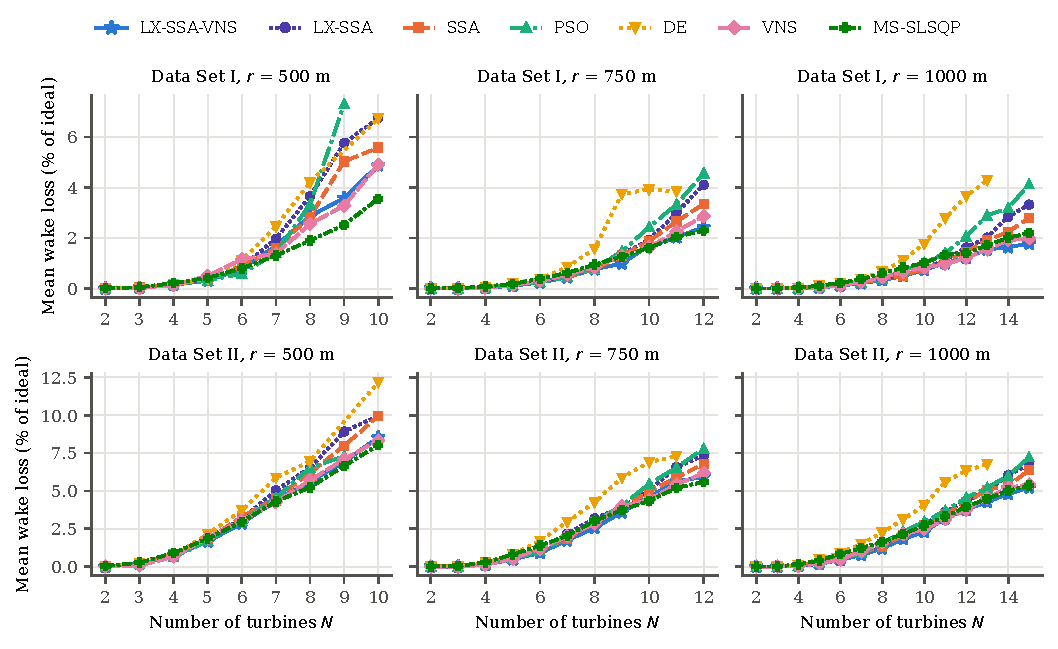
\includegraphics[width=\textwidth]{figures_final/wakeloss_vs_n.pdf}
\caption{Mean wake loss (percentage of the wake-free objective) of the feasible runs versus the prescribed number of turbines; a point is omitted when a method has no feasible run. \TBD{regenerate with SSA-VNS and constriction PSO}}
\label{fig:wakeloss}
\end{figure*}
\begin{figure*}[!t]
\centering
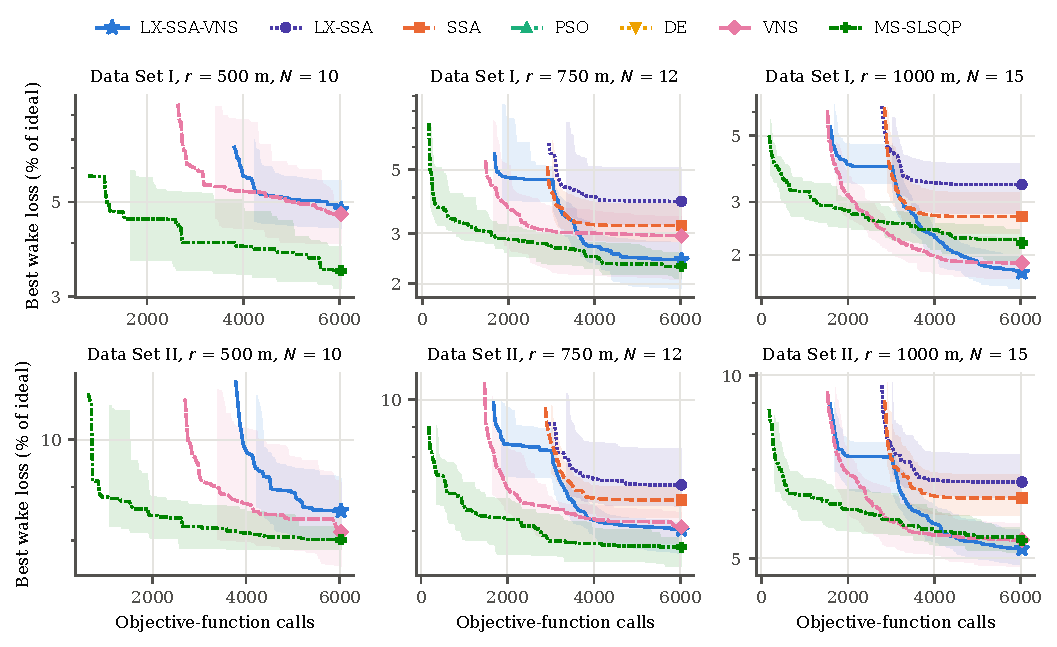
\includegraphics[width=\textwidth]{figures_final/convergence_max.pdf}
\caption{Convergence for the largest turbine count of each farm: median (line) and interquartile range (band) of the best feasible wake loss over the 30 runs versus the number of objective calls (logarithmic scale). A curve starts once at least half of the runs have found a feasible layout; the SSA-VNS curve switches from SSA to VNS at 3,030 calls. \TBD{regenerate with SSA-VNS and constriction PSO}}
\label{fig:conv-max}
\end{figure*}

Fig.~\ref{fig:wakeloss} shows how the wake loss depends on the case. It grows with $N$, falls as the farm becomes larger, and is higher for the broader wind rose of Data Set~II. For $N\le3$, all methods stay within \TBD{}\% of the wake-free objective. For 15 turbines in the 1000-m farm (Data Set~I), the mean wake loss is \TBD{}\% for SSA-VNS, \TBD{}\% for VNS, \TBD{}\% for MS-SLSQP, \TBD{}\% for SSA and \TBD{}\% for LX-SSA; for 12 turbines in the 750-m farm (Data Set~II), the corresponding values are \TBD{five values}. In the largest case of every farm, SSA-VNS reduces the mean wake loss of SSA by \TBD{range} percentage points.

SSA-VNS ends with a feasible layout in \TBD{}\% of all runs; the other methods reach \TBD{} (SSA), \TBD{} (LX-SSA), \TBD{} (PSO), \TBD{} (DE), \TBD{} (VNS) and \TBD{}\% (MS-SLSQP). The feasibility counts of the penalty-based methods are the same for both wind data sets, because as long as every candidate is infeasible, the penalty dominates $F_p$. In the densest cases (500~m, $N=10$), \TBD{feasibility of SSA at the switch and after VNS}.

Fig.~\ref{fig:conv-max} shows the effect of the second phase directly. Up to 3,030 calls, SSA-VNS runs a shortened SSA and is therefore behind the full SSA run. After the switch, its curve drops steeply, whereas SSA and LX-SSA stagnate. Over all feasible runs, the VNS phase removes on average \TBD{}\% (median \TBD{}\%) of the wake loss left at the end of the SSA phase, and it turns \TBD{} runs that were still infeasible at the switch into feasible ones. \TBD{comparison with VNS and MS-SLSQP convergence}.

\subsection{Ablation and Budget Split}
\label{sec:ablation}
\begin{table}[!t]
\centering
\caption{Ablation over the 68 Benchmark Cases (30 Seed-Paired Runs, 6,030 Calls). Top: Average Rank Among the Five Variants and Feasible Runs. Bottom: Contrasts of SSA-VNS, Cases in Which SSA-VNS Is Significantly Better / Not Different / Worse (Wilcoxon, Holm-Adjusted over the Four Contrasts of Each Case, $\alpha=0.05$), and Mean Difference of the Wake Loss (Percentage Points; Negative = SSA-VNS Better)}
\label{tab:ablation}
\scriptsize\setlength{\tabcolsep}{2.5pt}
\begin{tabular}{lcccc}
\toprule
Variant & Phase 1 & Phase 2 & Avg.\ rank & Feas.\ (\%) \\
\midrule
SSA-VNS & SSA & VNS & \TBD{} & \TBD{} \\
LX-SSA-VNS & LX-SSA & VNS & \TBD{} & \TBD{} \\
RS-VNS & random sampling & VNS & \TBD{} & \TBD{} \\
VNS & -- & VNS & \TBD{} & \TBD{} \\
SSA & SSA & -- & \TBD{} & \TBD{} \\
\bottomrule
\end{tabular}

\smallskip
\begin{tabular}{l>{\raggedright\arraybackslash}p{2.9cm}cc}
\toprule
SSA-VNS vs. & Isolates & W/T/L & Mean diff. \\
\midrule
SSA & VNS phase & \TBD{} & \TBD{} \\
VNS & swarm start vs.\ best initial point & \TBD{} & \TBD{} \\
RS-VNS & swarm vs.\ random sampling & \TBD{} & \TBD{} \\
LX-SSA-VNS & Laplace step in the hybrid & \TBD{} & \TBD{} \\
\bottomrule
\end{tabular}
\end{table}
\begin{figure*}[!t]
\centering
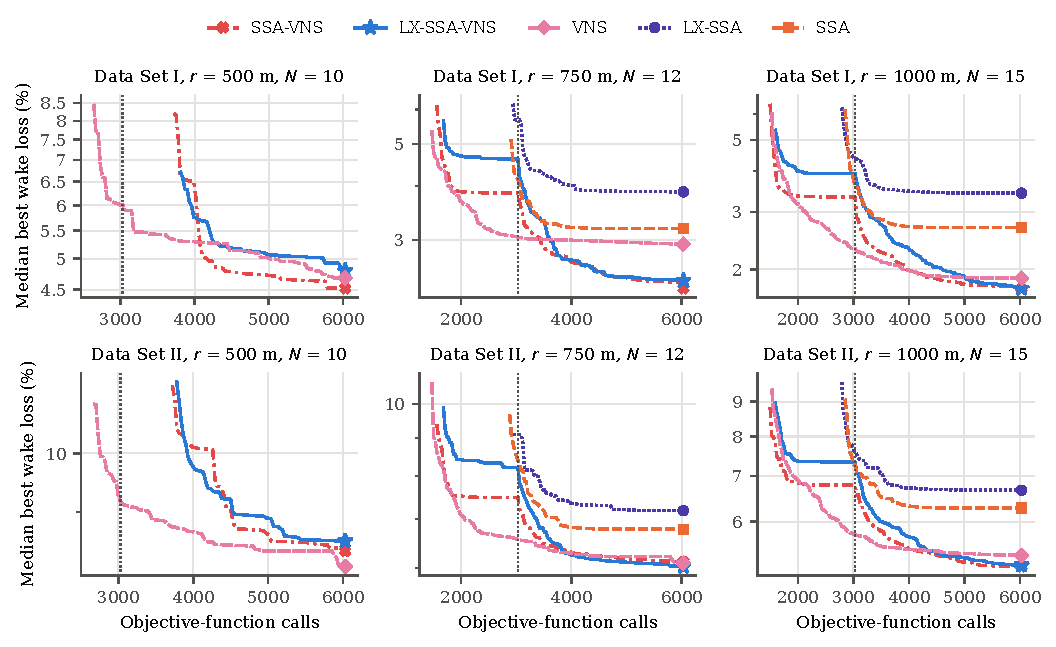
\includegraphics[width=\textwidth]{figures_final/ablation_convergence.pdf}
\caption{Ablation, largest turbine count of each farm: median best feasible wake loss over 30 runs versus objective calls for SSA, VNS, RS-VNS, LX-SSA-VNS and SSA-VNS (dotted line: switch to VNS at 3,030 calls). \TBD{regenerate with the five ablation variants}}
\label{fig:ablation}
\end{figure*}
\begin{table}[!t]
\centering
\caption{Sensitivity of SSA-VNS to the Budget Split (25\%, 50\% and 75\% of the 6,030 Calls for SSA): Mean Benchmark Objective of the Feasible Runs and Holm-Adjusted Wilcoxon $p$ of the 50\% Split Against the 25\% and 75\% Splits}
\label{tab:split}
\scriptsize\setlength{\tabcolsep}{2.5pt}
\begin{tabular}{cccccccc}
\toprule
DS & $r$ & $N$ & 25\% & 50\% & 75\% & $p$ (25) & $p$ (75) \\
\midrule
1 & 500 & 6 & \TBD{} & \TBD{} & \TBD{} & \TBD{} & \TBD{} \\
1 & 500 & 10 & \TBD{} & \TBD{} & \TBD{} & \TBD{} & \TBD{} \\
1 & 750 & 8 & \TBD{} & \TBD{} & \TBD{} & \TBD{} & \TBD{} \\
1 & 750 & 12 & \TBD{} & \TBD{} & \TBD{} & \TBD{} & \TBD{} \\
1 & 1000 & 10 & \TBD{} & \TBD{} & \TBD{} & \TBD{} & \TBD{} \\
1 & 1000 & 15 & \TBD{} & \TBD{} & \TBD{} & \TBD{} & \TBD{} \\
2 & 500 & 6 & \TBD{} & \TBD{} & \TBD{} & \TBD{} & \TBD{} \\
2 & 500 & 10 & \TBD{} & \TBD{} & \TBD{} & \TBD{} & \TBD{} \\
2 & 750 & 8 & \TBD{} & \TBD{} & \TBD{} & \TBD{} & \TBD{} \\
2 & 750 & 12 & \TBD{} & \TBD{} & \TBD{} & \TBD{} & \TBD{} \\
2 & 1000 & 10 & \TBD{} & \TBD{} & \TBD{} & \TBD{} & \TBD{} \\
2 & 1000 & 15 & \TBD{} & \TBD{} & \TBD{} & \TBD{} & \TBD{} \\
\bottomrule
\end{tabular}
\end{table}

To see where the improvement of SSA-VNS comes from, we compare it with four variants that each remove or replace one ingredient (Table~\ref{tab:ablation} and Fig.~\ref{fig:ablation}). The Friedman test over the five variants gives $\chi^2_F=$ \TBD{} (4 d.f., $p=$ \TBD{}), and SSA-VNS has the best average rank (\TBD{}).

Adding the VNS phase is the most important step: SSA-VNS beats SSA in \TBD{} cases and loses \TBD{}, and the mean wake loss falls by \TBD{} percentage points. Starting VNS from the SSA food source rather than from the best initial point \TBD{effect vs.\ VNS}. The random-multistart control RS-VNS spends the same 3,015 calls of Phase~1 on independent random layouts; \TBD{effect vs.\ RS-VNS and interpretation: does the swarm phase add value beyond a good random start?}.

The Laplace step did not help. Inside the hybrid, LX-SSA-VNS is \TBD{W/T/L} against SSA-VNS, with a mean wake-loss difference of \TBD{} percentage points in favor of SSA-VNS; without the VNS phase, LX-SSA is \TBD{W/T/L} against SSA. This is why the proposed method uses the standard SSA. The split of the budget between the two phases matters little (Table~\ref{tab:split}): \TBD{number of cases where 50\% is best, significant differences}.

\section{Results Beyond the Benchmark}
\label{sec:beyond}

\subsection{Feasibility-Preserving Initialization}
\label{sec:feasinit}
\begin{table}[!t]
\centering
\caption{Random vs.\ Feasibility-Preserving Initialization at 6,030 Calls: Mean Wake Loss (\%) over the Six Largest Benchmark Cases and Mean AEP Loss (\%) of the Horns Rev~1 16-Turbine Block, and Feasible Runs (\%)}
\label{tab:feasinit}
\scriptsize\setlength{\tabcolsep}{2.5pt}
\begin{tabular}{lcccccccc}
\toprule
& \multicolumn{4}{c}{Six largest cases} & \multicolumn{4}{c}{Horns Rev~1 block} \\
\cmidrule(lr){2-5}\cmidrule(lr){6-9}
& \multicolumn{2}{c}{Random} & \multicolumn{2}{c}{Feasible} & \multicolumn{2}{c}{Random} & \multicolumn{2}{c}{Feasible} \\
Method & Loss & Feas. & Loss & Feas. & Loss & Feas. & Loss & Feas. \\
\midrule
SSA-VNS & \TBD{} & \TBD{} & \TBD{} & \TBD{} & \TBD{} & \TBD{} & \TBD{} & \TBD{} \\
LX-SSA-VNS & \TBD{} & \TBD{} & \TBD{} & \TBD{} & \TBD{} & \TBD{} & \TBD{} & \TBD{} \\
RS-VNS & \TBD{} & \TBD{} & \TBD{} & \TBD{} & \TBD{} & \TBD{} & \TBD{} & \TBD{} \\
VNS & \TBD{} & \TBD{} & \TBD{} & \TBD{} & \TBD{} & \TBD{} & \TBD{} & \TBD{} \\
SSA & \TBD{} & \TBD{} & \TBD{} & \TBD{} & \TBD{} & \TBD{} & \TBD{} & \TBD{} \\
LX-SSA & \TBD{} & \TBD{} & \TBD{} & \TBD{} & \TBD{} & \TBD{} & \TBD{} & \TBD{} \\
PSO & \TBD{} & \TBD{} & \TBD{} & \TBD{} & \TBD{} & \TBD{} & \TBD{} & \TBD{} \\
DE & \TBD{} & \TBD{} & \TBD{} & \TBD{} & \TBD{} & \TBD{} & \TBD{} & \TBD{} \\
MS-SLSQP & \TBD{} & \TBD{} & \TBD{} & \TBD{} & \TBD{} & \TBD{} & \TBD{} & \TBD{} \\
\bottomrule
\end{tabular}
\end{table}

Table~\ref{tab:feasinit} compares random and feasibility-preserving initialization. \TBD{effect on feasibility rates, in particular for PSO and DE, which rarely reach feasibility from random starts in the dense cases}. \TBD{effect on wake loss and on the ranking; whether SSA-VNS keeps the best rank}.

\subsection{Budget Scaling}
\label{sec:budget}
\begin{table}[!t]
\centering
\caption{Budget Scaling: Average Rank over the Six Largest Benchmark Cases and Mean AEP Loss (\%) of the Horns Rev~1 16-Turbine Block at 6,030, 30,030 and 120,030 Calls (Random Initialization)}
\label{tab:budget}
\scriptsize\setlength{\tabcolsep}{2.5pt}
\begin{tabular}{lcccccc}
\toprule
& \multicolumn{3}{c}{Avg.\ rank (six cases)} & \multicolumn{3}{c}{Horns Rev~1 loss (\%)} \\
\cmidrule(lr){2-4}\cmidrule(lr){5-7}
Method & 6,030 & 30,030 & 120,030 & 6,030 & 30,030 & 120,030 \\
\midrule
SSA-VNS & \TBD{} & \TBD{} & \TBD{} & \TBD{} & \TBD{} & \TBD{} \\
LX-SSA-VNS & \TBD{} & \TBD{} & \TBD{} & \TBD{} & \TBD{} & \TBD{} \\
RS-VNS & \TBD{} & \TBD{} & \TBD{} & \TBD{} & \TBD{} & \TBD{} \\
VNS & \TBD{} & \TBD{} & \TBD{} & \TBD{} & \TBD{} & \TBD{} \\
SSA & \TBD{} & \TBD{} & \TBD{} & \TBD{} & \TBD{} & \TBD{} \\
LX-SSA & \TBD{} & \TBD{} & \TBD{} & \TBD{} & \TBD{} & \TBD{} \\
PSO & \TBD{} & \TBD{} & \TBD{} & \TBD{} & \TBD{} & \TBD{} \\
DE & \TBD{} & \TBD{} & \TBD{} & \TBD{} & \TBD{} & \TBD{} \\
MS-SLSQP & \TBD{} & \TBD{} & \TBD{} & \TBD{} & \TBD{} & \TBD{} \\
\bottomrule
\end{tabular}
\end{table}

Table~\ref{tab:budget} shows how the results change with the budget. \TBD{does the ranking change with 5$\times$ and 20$\times$ the budget; does the advantage of SSA-VNS over VNS, RS-VNS and MS-SLSQP grow or shrink; do PSO and DE become feasible}.

\subsection{Horns Rev~1 16-Turbine Block}
\label{sec:hornsrev-site}
\begin{table}[!t]
\centering
\caption{Horns Rev~1 16-Turbine Block (Wake-Free AEP 149.26 GWh/yr) at 6,030 Calls: AEP in GWh/yr, Mean (SD) over the Feasible Runs of 30 Seeds, Mean Wake Loss, Feasible Runs and Holm-Adjusted Wilcoxon $p$ of SSA-VNS vs.\ Each Method}
\label{tab:hr-site}
\scriptsize\setlength{\tabcolsep}{3pt}
\begin{tabular}{lcccc}
\toprule
Layout / method & AEP & Loss (\%) & Feas. & $p_{\rm Holm}$ \\
\midrule
Installed layout & 139.51 & 6.53 & -- & -- \\
\midrule
SSA-VNS & \TBD{} & \TBD{} & \TBD{} & -- \\
SSA & \TBD{} & \TBD{} & \TBD{} & \TBD{} \\
LX-SSA & \TBD{} & \TBD{} & \TBD{} & \TBD{} \\
PSO & \TBD{} & \TBD{} & \TBD{} & \TBD{} \\
DE & \TBD{} & \TBD{} & \TBD{} & \TBD{} \\
VNS & \TBD{} & \TBD{} & \TBD{} & \TBD{} \\
MS-SLSQP & \TBD{} & \TBD{} & \TBD{} & \TBD{} \\
\bottomrule
\end{tabular}
\end{table}

Table~\ref{tab:hr-site} gives the results for the 16-turbine block; the installed layout, a regular $7D$ grid, reaches 139.51~GWh/yr (wake loss 6.53\%). SSA-VNS attains \TBD{mean AEP, feasibility and significance against the other methods}. \TBD{whether PSO (constriction) and DE now find feasible layouts inside the parallelogram}. \TBD{whether any method improves on the installed layout at 6,030 calls and at the larger budgets of Section~\ref{sec:budget}}.

\subsection{IEA37 Case Study~1}
\label{sec:iea37}
\begin{table}[!t]
\centering
\caption{IEA37 Case Study~1, 16- and 36-Turbine Scenarios: AEP in MWh of the Best Run of Each Method at 6,030 and 30,030 Calls, Compared with the Example Layout and the Best Feasible Published Layout~\cite{Baker2019,IEA37repo}}
\label{tab:iea37}
\scriptsize\setlength{\tabcolsep}{2.5pt}
\begin{tabular}{lcccc}
\toprule
& \multicolumn{2}{c}{16 turbines ($r=1300$~m)} & \multicolumn{2}{c}{36 turbines ($r=2000$~m)} \\
\cmidrule(lr){2-3}\cmidrule(lr){4-5}
Method / source & 6,030 & 30,030 & 6,030 & 30,030 \\
\midrule
Example layout & \multicolumn{2}{c}{366,941.6} & \multicolumn{2}{c}{737,883.1} \\
Best feasible published$^{a}$ & \multicolumn{2}{c}{418,924.4} & \multicolumn{2}{c}{863,676.3} \\
\midrule
SSA-VNS & \TBD{} & \TBD{} & \TBD{} & \TBD{} \\
SSA & \TBD{} & \TBD{} & \TBD{} & \TBD{} \\
LX-SSA & \TBD{} & \TBD{} & \TBD{} & \TBD{} \\
PSO & \TBD{} & \TBD{} & \TBD{} & \TBD{} \\
DE & \TBD{} & \TBD{} & \TBD{} & \TBD{} \\
VNS & \TBD{} & \TBD{} & \TBD{} & \TBD{} \\
MS-SLSQP & \TBD{} & \TBD{} & \TBD{} & \TBD{} \\
\bottomrule
\multicolumn{5}{p{0.92\columnwidth}}{$^{a}$Participant~4 in both scenarios (SNOPT with wake expansion continuation \TBD{verify against Baker et al.\ (2019)}). A higher submitted AEP places turbines up to 3.5~m outside the boundary and is not counted.}
\end{tabular}
\end{table}

Table~\ref{tab:iea37} places our methods in the context of IEA37 Case Study~1, in which the participants chose their own optimizers and budgets~\cite{Baker2019}. Starting from the example layouts (366,941.6 and 737,883.1~MWh), the best feasible submitted layouts reach 418,924.4~MWh for 16 turbines and 863,676.3~MWh for 36 turbines. \TBD{rank of the best and mean SSA-VNS layouts among the submitted layouts; gap to the best feasible published layout at 6,030 and 30,030 calls}. Since most participants used gradient-based methods and budgets that are not reported in a comparable form, this comparison is indicative only.

\subsection{Comparison with Published Kusiak--Song Results}
\label{sec:literature}
The Kusiak--Song benchmark has been solved with evolution strategies~\cite{Kusiak2010}, ACO~\cite{Eroglu2012}, particle filtering~\cite{Eroglu2013} and biogeography-based optimization~\cite{Bansal2017}. \TBD{literature table pending author verification of the PDFs}

\subsection{Computational Cost}
\label{sec:runtime}
At equal numbers of objective calls, all methods need almost the same time: \TBD{ms per call for each method}. The objective evaluation dominates the cost, so neither the Laplace step nor the VNS bookkeeping adds a measurable overhead. One 6,030-call run of SSA-VNS takes \TBD{range}~s on average, depending on $N$.

\section{Sensitivity to the Modeling Assumptions}
\label{sec:robustness}
\subsection{Power Curve and Wake Model}
\label{sec:powercurve}
\label{sec:gaussian}
\begin{table*}[!t]
\centering
\caption{Robustness to the Benchmark Model: All Feasible Final Layouts Are Re-Evaluated (Not Re-Optimized). Change: Mean Relative Change of the Objective with Respect to the Benchmark Model; Average Rank of Each Method over the 68 Cases (Methods with at Least Five Feasible Runs); $\bar\tau$: Mean Kendall Correlation Between the Benchmark and Alternative Orderings Within a Case; ``Same Best'': Cases in Which the Best Method Is Unchanged}
\label{tab:robust-final}
\scriptsize\setlength{\tabcolsep}{3pt}
\begin{tabular}{lccccccccccc}
\toprule
& \multicolumn{2}{c}{Change (\%)} & \multicolumn{7}{c}{Average rank} & & \\
\cmidrule(lr){2-3}\cmidrule(lr){4-10}
Model & DS I & DS II & SSA-VNS & SSA & LX-SSA & PSO & DE & VNS & MS-SLSQP & $\bar\tau$ & Same best (\%) \\
\midrule
Benchmark (linear curve, Jensen) & +0.0 & +0.0 & \TBD{} & \TBD{} & \TBD{} & \TBD{} & \TBD{} & \TBD{} & \TBD{} & -- & -- \\
Cubic power curve & \TBD{} & \TBD{} & \TBD{} & \TBD{} & \TBD{} & \TBD{} & \TBD{} & \TBD{} & \TBD{} & \TBD{} & \TBD{} \\
Cubic curve with 25 m/s cut-out & \TBD{} & \TBD{} & \TBD{} & \TBD{} & \TBD{} & \TBD{} & \TBD{} & \TBD{} & \TBD{} & \TBD{} & \TBD{} \\
Gaussian wake ($K_{\rm G}=0.04$) & \TBD{} & \TBD{} & \TBD{} & \TBD{} & \TBD{} & \TBD{} & \TBD{} & \TBD{} & \TBD{} & \TBD{} & \TBD{} \\
\bottomrule
\end{tabular}
\end{table*}

We re-evaluated every feasible final layout of the main comparison, without re-optimization, with three alternative models: 1) a cubic power curve~\cite{Carrillo2013}, $f_{\rm c}(s)=P_{\text{rated}}(s^3-s_{\text{cut-in}}^3)/(s_{\text{rated}}^3-s_{\text{cut-in}}^3)$ between the cut-in and rated speeds; 2) the same curve with a 25~m/s cut-out; and 3) the Gaussian wake model of Bastankhah and Port\'e-Agel~\cite{Bastankhah2014},
\begin{align*}
\Delta_{ij}&=\Bigl(1-\sqrt{1-C_T/(8\sigma^2/D^2)}\Bigr)\exp\!\bigl(-v_{ij}^2/(2\sigma^2)\bigr),\\
\sigma/D&=K_{\rm G}\,d_{ij}/D+\epsilon,\\
\epsilon&=0.2\sqrt{\tfrac12(1+\sqrt{1-C_T})/\sqrt{1-C_T}},
\end{align*}
for turbines $i$ downstream of $j$, with $K_{\rm G}=0.04$, the lateral offset $v_{ij}$ of Definition~1, and the same superposition and Weibull scaling as the benchmark.

Table~\ref{tab:robust-final} shows two kinds of sensitivity. First, the absolute energy depends strongly on the model: the linear benchmark curve overstates the expected power relative to the cubic curve by \TBD{}\% for Data Set~I and \TBD{}\% for Data Set~II. The energy values in this paper should therefore be read as benchmark values and not as AEP predictions for a specific turbine. Second, the ranking of the algorithms is \TBD{stable/unstable} under the cubic curve ($\bar\tau=$ \TBD{}) and \TBD{} under the Gaussian model ($\bar\tau=$ \TBD{}; same best method in \TBD{}\% of the cases), because layouts optimized for the sharp Jensen wake cone are judged differently by a smooth Gaussian deficit. \TBD{rank of SSA-VNS under the Gaussian model}.

\subsection{Minimum Spacing}
\label{sec:spacing}
\begin{table}[!t]
\centering
\caption{Largest Turbine Count for Which a Layout Satisfying the Circular Boundary and the Minimum Spacing Was Constructed (Multi-Start Packing Search; Constructive Lower Bound), Compared with the Largest Tested $N$}
\label{tab:capacity}
\footnotesize
\begin{tabular}{ccccc}
\toprule
$r$ (m) & $4D$ & $5D$ & $6D$ & Largest \\
 & (308 m) & (385 m) & (462 m) & tested $N$ \\
\midrule
500 & 13 & 8 & 7 & 10 \\
750 & 26 & 19 & 13 & 12 \\
1000 & 42 & 29 & 21 & 15 \\
\bottomrule
\end{tabular}
\end{table}
\begin{table*}[!t]
\centering
\caption{Minimum-Spacing Sensitivity with LX-SSA and SSA (6,030 Calls, 30 Seed-Paired Runs per Cell): Mean Benchmark Objective, Wilcoxon Signed-Rank $p$ for LX-SSA vs.\ SSA, and Mean LX-SSA Wake Loss as a Percentage of the Ideal Objective at $4D$ and $6D$. A Superscript Gives the Number of Feasible Runs When Fewer Than 30}
\label{tab:spacing-authors}
\footnotesize\setlength{\tabcolsep}{3pt}
\begin{tabular}{ccccccccccccc}
\toprule
& & & \multicolumn{3}{c}{$4D$ (308 m)} & \multicolumn{3}{c}{$5D$ (385 m)} & \multicolumn{3}{c}{$6D$ (462 m)} & \\
\cmidrule(lr){4-6}\cmidrule(lr){7-9}\cmidrule(lr){10-12}
DS & $r$ (m) & $N$ & LX-SSA & SSA & $p$ & LX-SSA & SSA & $p$ & LX-SSA & SSA & $p$ & LX-SSA loss (\%) \\
\midrule
1 & 500 & 4 & 56078.8 & 56086.8 & 0.237 & 56082.4 & 56085.2 & 0.700 & 56075.5 & 56083.9 & 0.839 & 0.19 $\rightarrow$ 0.19 \\
1 & 750 & 8 & 111374.0 & 111506.5 & 0.245 & 111154.1 & 111163.4 & 0.871 & 110314.4$^{28}$ & 110847.5 & 0.021 & 0.88 $\rightarrow$ 1.85 \\
1 & 1000 & 8 & 111924.6 & 111947.1 & 0.887 & 111953.5 & 111946.4 & 0.777 & 111781.5 & 111964.7 & 0.005 & 0.39 $\rightarrow$ 0.52 \\
2 & 500 & 4 & 29004.2 & 29028.7 & 0.146 & 28999.5 & 29019.6 & 0.229 & 28981.8 & 28971.1 & 0.612 & 0.88 $\rightarrow$ 0.96 \\
2 & 750 & 8 & 56659.2 & 56806.2 & 0.061 & 56621.0 & 56673.3 & 0.584 & 56533.9$^{28}$ & 56690.6 & 0.038 & 3.18 $\rightarrow$ 3.47 \\
2 & 1000 & 8 & 57645.1 & 57739.3 & 0.084 & 57580.7 & 57655.7 & 0.140 & 57475.5 & 57587.2 & 0.114 & 1.50 $\rightarrow$ 1.79 \\
\bottomrule
\end{tabular}
\end{table*}

The $4D$ spacing is inherited from the benchmark literature, and we examined its influence in three ways. First, Table~\ref{tab:capacity} gives the largest turbine count for which a multi-start packing search constructed a feasible layout. These are constructive lower bounds, and the 500-m values agree with the known optimal circle-packing results. With $5D$ spacing, the 500-m farm holds at most 8 turbines and with $6D$ only 7, so the 500-m cases with $N\ge9$ (at $5D$) or $N\ge8$ (at $6D$) would be infeasible.

Second, the optimized layouts often lie on the $4D$ constraint. Of the \TBD{} feasible final layouts of the seven methods, \TBD{}\% also satisfy $5D$ and \TBD{}\% satisfy $6D$; for $N=6$--10 these shares fall to \TBD{}\% and \TBD{}\%, and for $N=11$--15 to \TBD{}\% and \TBD{}\%. Layouts optimized for $4D$ therefore cannot be transferred to a site with larger spacing requirements without re-optimization.

Third, we re-optimized six representative cases with LX-SSA and SSA at $5D$ and $6D$ (Table~\ref{tab:spacing-authors}). In the 750-m eight-turbine cases, the mean LX-SSA objective falls from $4D$ to $6D$ by 0.95\% (Data Set~I) and 0.22\% (Data Set~II), and the wake loss rises from 0.88\% to 1.85\% and from 3.18\% to 3.47\%. The spacing rule does not reverse the comparison between LX-SSA and SSA; in no cell is LX-SSA significantly better.

\subsection{Boundary Handling}
\label{sec:boundary}
All methods clip the coordinates to the bounding square and penalize turbines outside the circle (Section~\ref{sec:constraints}). An otherwise identical SSA that instead projects every turbine radially onto the circle attains higher mean objectives than the original SSA in six representative cases at 3,030 calls, by 26 to 649 objective units (Mann--Whitney $p<10^{-4}$ in every case). The boundary rule therefore has a noticeable effect, and we keep it fixed for all methods.

\section{Limitations}
\label{sec:limits}
Our results should be read within the following limits. The ablation shows that the gain of SSA-VNS comes mainly from \TBD{VNS phase / swarm start, according to the ablation}; the Laplace step of LX-SSA gave no measurable gain, either alone or inside the hybrid. In single cases, SSA-VNS and VNS differ significantly in only \TBD{} of the 68 cases.

The budget study covers budgets of up to 120,030 calls but only the six largest benchmark cases and the Horns Rev~1 block, and the largest farms studied have 36 turbines (IEA37 Case Study~1). Realistic farms with 80 or more turbines, where penalty-based search struggles to find feasible layouts, are outside the scope of this study. The VNS settings and the split $\omega=0.5$ are fixed defaults and were not tuned, and pseudo-gradient and surrogate-based methods are discussed but not benchmarked.

The Jensen model and the linear power curve are benchmark choices. The absolute energy depends strongly on them, \TBD{the ranking under the Gaussian model}, and we did not re-optimize the benchmark layouts with the alternative models. The $4D$ spacing and the boundary rule also affect the absolute results. Finally, $N$ is prescribed in every run, and terrain, mixed turbine types, collector cables, grid connection, noise and environmental constraints, and economic objectives are outside the scope of this study.

\section{Conclusion}
\label{sec:conclusion}
This work presents SSA-VNS, a two-phase algorithm for the continuous wind farm layout problem in which the standard salp swarm algorithm explores the layout space and the basic variable neighborhood search then refines the best layout found. We evaluated it on the Jensen--Weibull benchmark with explicit constraint handling against SSA, LX-SSA, PSO with constriction coefficients, DE, VNS and a multistart SLSQP solver on 68 cases at equal budgets, in an ablation, with feasibility-preserving initialization and larger budgets, on a 16-turbine block of the Horns Rev~1 offshore farm, and on the 16- and 36-turbine scenarios of IEA37 Case Study~1.

SSA-VNS obtained the best average rank (\TBD{}), was \TBD{significance summary} and returned a feasible layout in \TBD{}\% of the runs. The ablation showed that \TBD{contributions of the VNS phase, the swarm start and the comparison with RS-VNS}. The Laplace step of our earlier LX-SSA did not improve the results, either alone or inside the hybrid, so the standard SSA is the better first phase. \TBD{one sentence each on feasible initialization, budget scaling, Horns Rev~1 and IEA37}. The ranking of the methods was \TBD{} under a cubic power curve and \TBD{} under a Gaussian wake model.

In future work, we will study a switch between the two phases that is triggered by the stagnation of the swarm, investigate which properties of the swarm phase make it a good starting point for VNS, and extend the approach to larger farms and higher-fidelity wake and power models.

\section*{Acknowledgment}
\TBD{acknowledgment, or delete this section}

\section*{Data Availability}
The source code, the per-run results (including the final coordinates and convergence curves of all runs) and the scripts that generate all tables and figures are openly available at \TBD{Zenodo DOI}. The supplementary material contains the per-case results of the 68 benchmark cases (Tables~S1--S6), the coordinates of the best layouts, and additional convergence, distribution and layout figures. \TBD{assemble supplementary file}

\begin{thebibliography}{99}

\bibitem{Mosetti1994}
G. Mosetti, C. Poloni, and B. Diviacco, ``Optimization of wind turbine positioning in large windfarms by means of a genetic algorithm,'' \textit{J. Wind Eng. Ind. Aerodyn.}, vol. 51, no. 1, pp. 105--116, Jan. 1994, doi: 10.1016/0167-6105(94)90080-9.

\bibitem{Grady2005}
S. A. Grady, M. Y. Hussaini, and M. M. Abdullah, ``Placement of wind turbines using genetic algorithms,'' \textit{Renew. Energy}, vol. 30, no. 2, pp. 259--270, Feb. 2005, doi: 10.1016/j.renene.2004.05.007.

\bibitem{Ozturk2004}
U. A. Ozturk and B. A. Norman, ``Heuristic methods for wind energy conversion system positioning,'' \textit{Electr. Power Syst. Res.}, vol. 70, no. 3, pp. 179--185, Aug. 2004, doi: 10.1016/j.epsr.2003.12.006.

\bibitem{Lackner2007}
M. A. Lackner and C. N. Elkinton, ``An analytical framework for offshore wind farm layout optimization,'' \textit{Wind Eng.}, vol. 31, no. 1, pp. 17--31, Jan. 2007, doi: 10.1260/030952407780811401.

\bibitem{Mora2007}
J. Castro Mora, J. M. Calero Bar\'on, J. M. Riquelme Santos, and M. Burgos Pay\'an, ``An evolutive algorithm for wind farm optimal design,'' \textit{Neurocomputing}, vol. 70, no. 16--18, pp. 2651--2658, Oct. 2007, doi: 10.1016/j.neucom.2006.05.017.

\bibitem{Huang2007}
H.-S. Huang, ``Distributed genetic algorithm for optimization of wind farm annual profits,'' in \textit{Proc. Int. Conf. Intell. Syst. Appl. Power Syst. (ISAP)}, Kaohsiung, Taiwan, Nov. 2007, pp. 1--6, doi: 10.1109/ISAP.2007.4441654.

\bibitem{Elkinton2008}
C. N. Elkinton, J. F. Manwell, and J. G. McGowan, ``Algorithms for offshore wind farm layout optimization,'' \textit{Wind Eng.}, vol. 32, no. 1, pp. 67--84, Jan. 2008, doi: 10.1260/030952408784305877.

\bibitem{Bilbao2009}
M. Bilbao and E. Alba, ``Simulated annealing for optimization of wind farm annual profit,'' in \textit{Proc. 2nd Int. Symp. Logistics Ind. Informat. (LINDI)}, Linz, Austria, Sep. 2009, pp. 1--5, doi: 10.1109/LINDI.2009.5258656.

\bibitem{Rivas2009}
R. A. Rivas, J. Clausen, K. S. Hansen, and L. E. Jensen, ``Solving the turbine positioning problem for large offshore wind farms by simulated annealing,'' \textit{Wind Eng.}, vol. 33, no. 3, pp. 287--297, May 2009, doi: 10.1260/0309-524X.33.3.287.

\bibitem{Emami2010}
A. Emami and P. Noghreh, ``New approach on optimization in placement of wind turbines within wind farm by genetic algorithms,'' \textit{Renew. Energy}, vol. 35, no. 7, pp. 1559--1564, Jul. 2010, doi: 10.1016/j.renene.2009.11.026.

\bibitem{Sisbot2010}
S. \c{S}i\c{s}bot, \"O. Turgut, M. Tun\c{c}, and \"U. \c{C}amdal\i, ``Optimal positioning of wind turbines on G\"ok\c{c}eada using multi-objective genetic algorithm,'' \textit{Wind Energy}, vol. 13, no. 4, pp. 297--306, May 2010, doi: 10.1002/we.339.

\bibitem{Kusiak2010}
A. Kusiak and Z. Song, ``Design of wind farm layout for maximum wind energy capture,'' \textit{Renew. Energy}, vol. 35, no. 3, pp. 685--694, Mar. 2010, doi: 10.1016/j.renene.2009.08.019.

\bibitem{Eroglu2012}
Y. Ero\u{g}lu and S. U. Se\c{c}kiner, ``Design of wind farm layout using ant colony algorithm,'' \textit{Renew. Energy}, vol. 44, pp. 53--62, Aug. 2012, doi: 10.1016/j.renene.2011.12.013.

\bibitem{Eroglu2013}
Y. Ero\u{g}lu and S. U. Se\c{c}kiner, ``Wind farm layout optimization using particle filtering approach,'' \textit{Renew. Energy}, vol. 58, pp. 95--107, Oct. 2013, doi: 10.1016/j.renene.2013.02.019.

\bibitem{Samorani2013}
M. Samorani, ``The wind farm layout optimization problem,'' in \textit{Handbook of Wind Power Systems}, P. M. Pardalos, S. Rebennack, M. V. F. Pereira, N. A. Iliadis, and V. Pappu, Eds. Berlin, Germany: Springer, 2013, pp. 21--38, doi: 10.1007/978-3-642-41080-2\_2.

\bibitem{Bansal2017}
J. C. Bansal and P. Farswan, ``Wind farm layout using biogeography based optimization,'' \textit{Renew. Energy}, vol. 107, pp. 386--402, Jul. 2017, doi: 10.1016/j.renene.2017.01.064.

\bibitem{Srikakulapu2018}
R. Srikakulapu and U. Vinatha, ``Optimized design of collector topology for offshore wind farm based on ant colony optimization with multiple travelling salesman problem,'' \textit{J. Mod. Power Syst. Clean Energy}, vol. 6, no. 6, pp. 1181--1192, Nov. 2018, doi: 10.1007/s40565-018-0386-4.

\bibitem{Ju2019}
X. Ju and F. Liu, ``Wind farm layout optimization using self-informed genetic algorithm with information guided exploitation,'' \textit{Appl. Energy}, vol. 248, pp. 429--445, Aug. 2019, doi: 10.1016/j.apenergy.2019.04.084.

\bibitem{Jin2019}
R. Jin, P. Hou, G. Yang, Y. Qi, C. Chen, and Z. Chen, ``Cable routing optimization for offshore wind power plants via wind scenarios considering power loss cost model,'' \textit{Appl. Energy}, vol. 254, Art. no. 113719, Nov. 2019, doi: 10.1016/j.apenergy.2019.113719.

\bibitem{Hou2019}
P. Hou, J. Zhu, K. Ma, G. Yang, W. Hu, and Z. Chen, ``A review of offshore wind farm layout optimization and electrical system design methods,'' \textit{J. Mod. Power Syst. Clean Energy}, vol. 7, no. 5, pp. 975--986, Sep. 2019, doi: 10.1007/s40565-019-0550-5.

\bibitem{Dhiman2020}
H. S. Dhiman, D. Deb, and A. M. Foley, ``Lidar assisted wake redirection in wind farms: A data driven approach,'' \textit{Renew. Energy}, vol. 152, pp. 484--493, Jun. 2020, doi: 10.1016/j.renene.2020.01.027.

\bibitem{Nagpal2021}
S. V. Nagpal, M. V. Liu, and C. L. Anderson, ``A comparison of deterministic refinement techniques for wind farm layout optimization,'' \textit{Renew. Energy}, vol. 168, pp. 581--592, May 2021, doi: 10.1016/j.renene.2020.12.043.

\bibitem{Asaah2021}
P. Asaah, L. Hao, and J. Ji, ``Optimal placement of wind turbines in wind farm layout using particle swarm optimization,'' \textit{J. Mod. Power Syst. Clean Energy}, vol. 9, no. 2, pp. 367--375, Mar. 2021, doi: 10.35833/MPCE.2019.000087.

\bibitem{Bai2022}
F. Bai, X. Ju, S. Wang, W. Zhou, and F. Liu, ``Wind farm layout optimization using adaptive evolutionary algorithm with Monte Carlo tree search reinforcement learning,'' \textit{Energy Convers. Manage.}, vol. 252, Art. no. 115047, Jan. 2022, doi: 10.1016/j.enconman.2021.115047.

\bibitem{Cazzaro2022}
D. Cazzaro and D. Pisinger, ``Variable neighborhood search for large offshore wind farm layout optimization,'' \textit{Comput. Oper. Res.}, vol. 138, Art. no. 105588, Feb. 2022, doi: 10.1016/j.cor.2021.105588.

\bibitem{Quaeghebeur2021}
E. Quaeghebeur, R. Bos, and M. B. Zaaijer, ``Wind farm layout optimization using pseudo-gradients,'' \textit{Wind Energy Sci.}, vol. 6, no. 3, pp. 815--839, Jun. 2021, doi: 10.5194/wes-6-815-2021.

\bibitem{Tao2020}
S. Tao, Q. Xu, A. Feij\'oo, G. Zheng, and J. Zhou, ``Wind farm layout optimization with a three-dimensional Gaussian wake model,'' \textit{Renew. Energy}, vol. 159, pp. 553--569, Oct. 2020, doi: 10.1016/j.renene.2020.06.003.

\bibitem{Yang2023}
K. Yang, X. Deng, Z. Ti, S. Yang, S. Huang, and Y. Wang, ``A data-driven layout optimization framework of large-scale wind farms based on machine learning,'' \textit{Renew. Energy}, vol. 218, Art. no. 119240, Dec. 2023, doi: 10.1016/j.renene.2023.119240.

\bibitem{Wang2024}
Z. Wang, Y. Tu, K. Zhang, Z. Han, Y. Cao, and D. Zhou, ``An optimization framework for wind farm layout design using CFD-based Kriging model,'' \textit{Ocean Eng.}, vol. 293, Art. no. 116644, Feb. 2024, doi: 10.1016/j.oceaneng.2023.116644.

\bibitem{Yang2024}
S. Yang, X. Deng, and K. Yang, ``Machine-learning-based wind farm optimization through layout design and yaw control,'' \textit{Renew. Energy}, vol. 224, Art. no. 120161, Apr. 2024, doi: 10.1016/j.renene.2024.120161.

\bibitem{Li2025}
P. Li, Y. Che, A. Hua, L. Wang, M. Zheng, and X. Guo, ``A data-physics hybrid-driven layout optimization framework for large-scale wind farms,'' \textit{Appl. Energy}, vol. 392, Art. no. 125908, 2025, doi: 10.1016/j.apenergy.2025.125908.

\bibitem{Baker2019}
N. F. Baker, A. P. J. Stanley, J. J. Thomas, A. Ning, and K. Dykes, ``Best practices for wake model and optimization algorithm selection in wind farm layout optimization,'' in \textit{Proc. AIAA SciTech Forum}, San Diego, CA, USA, Jan. 2019, Paper AIAA 2019-0540, doi: 10.2514/6.2019-0540.

\bibitem{IEA37repo}
N. F. Baker \textit{et al.}, ``IEA Wind Task 37 wind farm layout optimization case studies: Case files and submitted results.'' [Online]. Available: \url{https://github.com/IEAWindTask37/iea37-wflo-casestudies}

\bibitem{Mirjalili2017}
S. Mirjalili, A. H. Gandomi, S. Z. Mirjalili, S. Saremi, H. Faris, and S. M. Mirjalili, ``Salp swarm algorithm: A bio-inspired optimizer for engineering design problems,'' \textit{Adv. Eng. Softw.}, vol. 114, pp. 163--191, Dec. 2017, doi: 10.1016/j.advengsoft.2017.07.002.

\bibitem{Solanki2023}
P. Solanki and K. Deep, ``Laplacian salp swarm algorithm for continuous optimization,'' \textit{Int. J. Syst. Assur. Eng. Manag.}, 2023, doi: 10.1007/s13198-023-01935-y.

\bibitem{Kennedy1995}
J. Kennedy and R. Eberhart, ``Particle swarm optimization,'' in \textit{Proc. IEEE Int. Conf. Neural Netw. (ICNN)}, Perth, WA, Australia, Nov. 1995, vol. 4, pp. 1942--1948, doi: 10.1109/ICNN.1995.488968.

\bibitem{Clerc2002}
M. Clerc and J. Kennedy, ``The particle swarm---Explosion, stability, and convergence in a multidimensional complex space,'' \textit{IEEE Trans. Evol. Comput.}, vol. 6, no. 1, pp. 58--73, Feb. 2002, doi: 10.1109/4235.985692.

\bibitem{Poli2009}
R. Poli, ``Mean and variance of the sampling distribution of particle swarm optimizers during stagnation,'' \textit{IEEE Trans. Evol. Comput.}, vol. 13, no. 4, pp. 712--721, Aug. 2009, doi: 10.1109/TEVC.2008.2011744.

\bibitem{Storn1997}
R. Storn and K. Price, ``Differential evolution---A simple and efficient heuristic for global optimization over continuous spaces,'' \textit{J. Global Optim.}, vol. 11, no. 4, pp. 341--359, Dec. 1997, doi: 10.1023/A:1008202821328.

\bibitem{Mladenovic1997}
N. Mladenovi\'c and P. Hansen, ``Variable neighborhood search,'' \textit{Comput. Oper. Res.}, vol. 24, no. 11, pp. 1097--1100, Nov. 1997, doi: 10.1016/S0305-0548(97)00031-2.

\bibitem{Hansen2001}
P. Hansen and N. Mladenovi\'c, ``Variable neighborhood search: Principles and applications,'' \textit{Eur. J. Oper. Res.}, vol. 130, no. 3, pp. 449--467, May 2001, doi: 10.1016/S0377-2217(00)00100-4.

\bibitem{Mladenovic2008}
N. Mladenovi\'c, M. Dra\v{z}i\'c, V. Kova\v{c}evi\'c-Vuj\v{c}i\'c, and M. \v{C}angalovi\'c, ``General variable neighborhood search for the continuous optimization,'' \textit{Eur. J. Oper. Res.}, vol. 191, no. 3, pp. 753--770, Dec. 2008, doi: 10.1016/j.ejor.2006.12.064.

\bibitem{Jensen1983}
N. O. Jensen, ``A note on wind generator interaction,'' Ris\o\ Nat. Lab., Roskilde, Denmark, Tech. Rep. Ris\o-M-2411, 1983.

\bibitem{Katic1986}
I. Kati\'c, J. H\o jstrup, and N. O. Jensen, ``A simple model for cluster efficiency,'' in \textit{Proc. Eur. Wind Energy Assoc. Conf. Exhib. (EWEC)}, Rome, Italy, Oct. 1986, vol. 1, pp. 407--410.

\bibitem{Cao2022}
L. Cao, M. Ge, X. Gao, B. Du, B. Li, Z. Huang, and Y. Liu, ``Wind farm layout optimization to minimize the wake induced turbulence effect on wind turbines,'' \textit{Appl. Energy}, vol. 323, Art. no. 119599, Oct. 2022, doi: 10.1016/j.apenergy.2022.119599.

\bibitem{Stroock1999}
D. W. Stroock, \textit{A Concise Introduction to the Theory of Integration}, 3rd ed. Boston, MA, USA: Birkh\"auser, 1999.

\bibitem{Deep2007}
K. Deep and M. Thakur, ``A new crossover operator for real coded genetic algorithms,'' \textit{Appl. Math. Comput.}, vol. 188, no. 1, pp. 895--911, May 2007, doi: 10.1016/j.amc.2006.10.047.

\bibitem{Kraft1988}
D. Kraft, ``A software package for sequential quadratic programming,'' DFVLR, Inst. f\"ur Dynamik der Flugsysteme, Oberpfaffenhofen, Germany, Tech. Rep. DFVLR-FB 88-28, 1988.

\bibitem{Holm1979}
S. Holm, ``A simple sequentially rejective multiple test procedure,'' \textit{Scand. J. Statist.}, vol. 6, no. 2, pp. 65--70, 1979.

\bibitem{Demsar2006}
J. Dem\v{s}ar, ``Statistical comparisons of classifiers over multiple data sets,'' \textit{J. Mach. Learn. Res.}, vol. 7, pp. 1--30, Jan. 2006.

\bibitem{PyWake}
DTU Wind Energy, ``PyWake: Open-source static wake modeling framework,'' Python package \texttt{py\_wake}, ver. 2.6.20 (Horns Rev~1 site data in \texttt{py\_wake/examples/data/hornsrev1.py}), MIT License. [Online]. Available: \url{https://gitlab.windenergy.dtu.dk/TOPFARM/PyWake}

\bibitem{Carrillo2013}
C. Carrillo, A. F. Obando Monta\~no, J. Cidr\'as, and E. D\'iaz-Dorado, ``Review of power curve modelling for wind turbines,'' \textit{Renew. Sustain. Energy Rev.}, vol. 21, pp. 572--581, May 2013, doi: 10.1016/j.rser.2013.01.012.

\bibitem{Bastankhah2014}
M. Bastankhah and F. Port\'e-Agel, ``A new analytical model for wind-turbine wakes,'' \textit{Renew. Energy}, vol. 70, pp. 116--123, Oct. 2014, doi: 10.1016/j.renene.2014.01.029.

\end{thebibliography}

\begin{IEEEbiographynophoto}{Prince Solanki}
\TBD{biography: degrees, institutions, research interests}
\end{IEEEbiographynophoto}

\begin{IEEEbiographynophoto}{Pulkit Dwivedi}
\TBD{biography}
\end{IEEEbiographynophoto}

\begin{IEEEbiographynophoto}{Vanita Garg}
\TBD{biography}
\end{IEEEbiographynophoto}

\begin{IEEEbiographynophoto}{Vinay Shukla}
\TBD{biography}
\end{IEEEbiographynophoto}

\end{document}
